\documentclass[a4paper,  11pt]{ctexart}
\usepackage{srcltx,graphicx}
\usepackage{amsmath, amssymb, amsthm}
\usepackage[usenames,dvipsnames]{color}   % 支持彩色
\usepackage{color}
\usepackage{xcolor}
\usepackage{colortbl}
\usepackage{lscape}
\usepackage{multirow}
\usepackage{psfrag}
\usepackage{diagbox}
\usepackage[hang]{subfigure}
\usepackage{listings}
\usepackage{float}
\usepackage[colorlinks,linkcolor=black,anchorcolor=blue,citecolor=green]{hyperref}

\newtheorem{theorem}{Theorem}
\newtheorem{lemma}{Lemma}
\newtheorem{definition}{Definition}
\newtheorem{comment}{Comment}
\newtheorem{conjecture}{Conjecture}

\newcommand\bbR{\mathbb{R}}
\newcommand\bbN{\mathbb{N}}
\newcommand\bbC{\mathbb{C}}
\newcommand\bx{\boldsymbol{x}}
\newcommand\dd{\,\mathrm{d}}

\newcommand\diag{\mathrm{diag}}
\newcommand\tr{\mthrm{tr}}

\setlength{\oddsidemargin}{0cm}
\setlength{\evensidemargin}{0cm}
\setlength{\textwidth}{150mm}
\setlength{\textheight}{230mm}
%========= 定义颜色 ===================================
\definecolor{blueblack}{cmyk}{0,0,0,0.35}%浅黑
\definecolor{darkblue}{cmyk}{1,0,0,0}%纯蓝
\definecolor{lightblue}{cmyk}{0.15,0,0,0}%浅蓝
\definecolor{shadecolor}{rgb}{0.90,0.90,0.90}

\newcommand\note[2]{{{\bf #1}\color{red} [ {\it #2} ]}}
%\newcommand\note[2]{{ #1 }} % using this line in the formal version

\newcommand\pd[2]{\dfrac{\partial {#1}}{\partial {#2}}}
\newcommand\od[2]{\dfrac{\dd {#1}}{\dd {#2}}}
\newcommand{\bm}[1]{\mbox{\boldmath{$#1$}}}
%========== 插入C++程序 =====================================
\lstset{language=C++}%这条命令可以让LaTeX排版时将C++键字突出显示
\lstset{breaklines}%这条命令可以让LaTeX自动将长的代码行换行排版
\lstset{extendedchars=false}%这一条命令可以解决代码跨页时,章节标题,页眉等汉字不显示的问题
\lstset{                       
    backgroundcolor=\color{shadecolor},
    basicstyle=\footnotesize\ttfamily,
    breakatwhitespace=false,
    captionpos=b,
 %   commentstyle=\color{darkblue},
    directivestyle=\color{blue},
    frame=single,%shadowbox
    framerule=0pt,
    keywordstyle=\color{blue}\bfseries,
    morekeywords={*,define,*,include\dots},
    numbersep=5pt,
 %   rulesepcolor=\color{red!20!green!20!blue!20},
    showspaces=false,
    showstringspaces=false,
    showtabs=false,
    stepnumber=2,
    stringstyle=\color{purple},
    tabsize=4,
    title=\lstname
}
\newcommand\inputccode[1]{\lstinputlisting{#1}}
%========== 插入C++程序结束 =================================

\begin{document}
\title{Gmsh初步学习 \\ 并行计算第一次作业}
\author{郑灵超}
\maketitle
\tableofcontents
\newpage
\section{Gmsh软件介绍}
\subsection{软件简介}
Gmsh是一款内嵌了CAD和后处理的三维有限元网格生成器。它能提供一种快速、轻
便、方便使用且有良好的可视化效果的网格生成工具。 

Gmsh主要有四个模块:几何体,网格,求解器和后处理,
在本报告中,我们将着重关心Gmsh中几何体的生成、网格的剖分,以及利用Gmsh
生成的网格结合AFEPack软件包进行有限元问题的求解。

本报告只是作者学习Gmsh软件的一些经验,纰漏之处在所难免,读者可以通过下
载Gmsh官方帮助文档
(http://gmsh.info/doc/texinfo/gmsh.pdf)获取更多信息。
\subsection{软件安装}
Gmsh的安装途径十分简单
\begin{itemize}
	\item 直接在ubuntu源中安装:终端输入 sudo apt-get install gmsh 即
		可。
	\item 在Gmsh官网(http://gmsh.info)下载软件包,解压后可以直接运行bin
	文件夹中的gmsh文件。
\end{itemize}
\subsection{软件使用方式}
\begin{itemize}
		\item 直接在终端输入gmsh,打开图形界面,之后可以生成新的文件或
			者在图形界面中打开指定的文件。
		\item 在命令行输入gmsh file,打开图形界面并载入制定文件。
		\item 通过命令行模式执行,例如\\
			 >gmsh t1.geo -2 \\
			 将会对指定文件t1.geo进行2维的网格剖分。
\end{itemize}
\par
关于软件使用形式的
\par
由于实际问题中结构体(点,线,面,体)的数目较多,在使用中我们建议
自己撰写或用生成geo文件,再用gmsh打开并操作。 
\subsection{Gmsh的优势与不足}
\subsubsection{Gmsh的优势}
\begin{itemize}
	\item 能够较快地描述几何体。
	\item 能够确定几何体的参数。
	\item 可以比较容易地生成一些简单的1D,2D,3D有限元网格,并与CAD软件
		有着较好的适应性。
	\item 可以精细地控制网格尺寸。
	\item 可以通过现有几何体的变换得到新的几何体。
	\item 自带了有限元的求解器。
\end{itemize}
\subsubsection{Gmsh的不足}
\begin{itemize}
	\item 用于描述几何体的方法——BRep approach在处理大规模模型时会不再
		方便。
	\item Gmsh生成的网格较为有限,只能剖分适合有限元方法的网格。
	\item Gmsh使用的文件,例如.geo文件的语言稍显落后,例如循环系统
		较为简陋,没有自定义的宏和局部变量。
	\item Gmsh没有撤销操作,将会带来一些不便。
\end{itemize}
\newpage
\section{几何结构的构造}
几何结构是Gmsh中最基本的元素,之后的网格剖分和方程计算都将基于构造好的
几何体。Gmsh不仅可以让用户自己从点开始生成几何体,也可以基于已有的几何
体经过变换和拉伸得到。

下面我们介绍一些最基本的几何结构的生成方式以及它们的作用和变换
形式。

\subsection{Point(点)}
\begin{itemize}
\item
~\verb|Point(n)={x,y,z,lc};|~ \\
这个命令可以在坐标
$(x,y,z)$处插入一个编号为$n$的点;$lc$是特征尺度,表示该点所属
网格的尺度,用于控制网格的疏密程度,$lc$可以省略。
\end{itemize}
\subsection{Line(线)}
\begin{itemize}
		\item 
~\verb|Line(n)={n1,n2};|~ \\
可以生成一条从第$n_1$号点到$n_2$号点的线段,线段编号为$n$。
\item 
	~\verb|Circle(n)={n1,n2,n3 }|~;  \\
	可以生成一条弧度小于$\pi$的圆弧,圆弧的圆心编号为
	$n_2$,起点编号为$n_1$,终点编号为$n_3$。
\end{itemize}
\subsection{Loop(环)}
Loop是Gmsh的几何结构相对于传统的欧式几何结构的不同之处,分为Line Loop
和Surface Loop。其中Line Loop可以用来定义面,而Surface Loop可以用于定义
体,此处我们先介绍Line Loop的产生。\par
~\verb|Line Loop(n)={expression list};|~ \par
用于产生 line loop. 其中$n$为line loop的编号,右端的experssion list包
含所有构成这个line loop的线。构成line loop的所有line必须是封闭且统一方
向的。
\subsection{Surface(面)}
\begin{itemize}
	\item ~\verb|Plane Surface(n)={expression list};|~ \\
		用于生成一个平面区域,其中$n$为区域编号,右端的expression 包含
		了若干个Line Loop,其中第一个Line Loop 是产生该区域的外边界
		,其余Line Loop为该区域的内边界(洞)。
\item ~\verb|Ruled Surface(n)={expression list} <In	Sphere{expression}>;|~ \\
		用于生成一个直纹曲面,其中$n$和expression list与Plane Surface中的
		相同,分别为编号和Line Loop; <> 中为可选的参数,表示该曲面限定
		在一个球面上并指定球心点编号。
	\item ~\verb|Surface Loop(n)={expression list};|~ \\
		用于生成surface loop,以构造体。其中$n$为surface loop的编号,
		右边为构成这个surface loop的所有面的编号,右边参数要保证
		surface loop是封闭的且自洽的(所有面法向指向同一个区域)。
	\item ~\verb|Compound Surface(n)={expression list};|~ \\
		用于生成一个复合平面。复合平面由若干平面组成,这些平面在网格剖
		分的时候被视为同一个平面(同一个网格可能跨过平面边界)。
\end{itemize}
\subsection{Volume(体)}
\begin{itemize}
	\item ~\verb|Volume(n)={expression list};|~ \\
		可以创建一个体。与创建面类似,expression list包含若干个Surface
		Loop,其中第一个为该几何体的外边界,其余几个为内边界(孔)。
	\item ~\verb|Compound Volume(n)={expression list};|~ \\
		可以创建一个组合的几何体。与组合面类似,组合体在进行网格剖分的
		时候网格可以跨越边界。
\end{itemize}
\subsection{Extrusions}
通过Extrude命令,我们可以从点生成线,从线生成面,从面生成几何体。
\begin{itemize}
	\item ~\verb|Extrude {x,y,z} {extrude list};|~ \\
		使得将extrude list中的元素沿着$(x,y,z)$方向移动对应距离,并将
		初始位置和最终位置对应连接。\\
		例如如果作用于点,生成的就是线;作用于线,生成的就是面;作用于
		面,生成的就是几何体。
	\item 
~\verb|Extrude{{x1,y1,z1},{x2,y2,z2},theta}{extrude list};|~\\
		将Extrude list中所有元素进行旋转操作,并根据轨迹生成新的几何结
		构。其中$(x_1,x_2,x_3)$给出了旋转轴的方向,
		$(x_2,y_2,z_2)$给出了旋转轴上的一个点,$\theta$给出了旋转角度
		(弧度)。
    \item 
~\verb|Extrude {{x,y,z},{x1,y1,z1},{x2,y2,z2},theta}{extrude list}; |~\\
		将Extrude list中的元素进行平移加旋转操作,平移和旋转的参数分别
		由$(x,y,z)$和$(x_1,y_1,z_1),(x_2,y_2,z_2),\theta$给出,规则与
		前文一致。
\end{itemize}
\subsection{Transformations}
Transformation作用于几何体将不再生成轨迹,而只是生成结果,默认将原数据
覆盖,也可以生成一个复制品(利用Duplicata命令)。
\begin{itemize}
	\item ~\verb|Dilate {{x,y,z},alpha}{transform list};|~ \\
		将transform list所有元素进行放缩,
		其中$(x,y,z)$ 给出了位似变换的方向,
		而$\alpha$给出放缩的比例。
	\item 
	~\verb|Rotate {{x1,y1,z1},{x2,y2,z2},theta}{transform list}; |~ \\
		将transform list所有元素进行旋转变换。其中
		$x_1,y_1,z_1,x_2,y_2,z_2,\theta$确定了旋转的参数,形式与
		Extrude中的旋转相同。
	\item 
	~\verb|Symmetry {a,b,c,d} { transform list };|~\\
		将transform list中所有元素进行对称操作。其中$a,b,c,d$给出了
		对称平面方程的四个系数。
	\item ~\verb|Translate {x,y,z} {transform list};|~ \\
		将transform list中所有元素沿着向量$(x,y,z)$平移。
	\item ~\verb|Boundary { transform list};|~ \\
		返回transform list中所有元素的边界。
	\item ~\verb|CombinedBoundary { transform list };|~ \\
		返回transform list所有元素总的边界。
\end{itemize}
\subsection{Physical entity(物理实体)}
由于完全使用Element entities将带来一些不便:
\begin{itemize}
	\item 网格元素不能被复制。
	\item 网格元素的节点编号完全由他们的“父”结构决定,而且难以修改。
	\item 隶属于不同元素结构体的一些元素不能被同一种数学物理的形式表出
		,如狄利克雷边界条件。
\end{itemize}
基于以上原因,在实际应用中需要引入一些物理实体。\par
 ~\verb|Physical Point(n) = { expression list }; |~ \\
 其中$n$为物理实体的编号,右端的 expression list 包括所有将被
 囊括到这个物理点的元素点(Element Point)的编号。
\newpage
 \section{网格生成}
\subsection{二维网格}
\subsubsection{二维三角形网格}
对于Surface,Gmsh默认将其剖分为三角形网格,因此二维无结构三角形网格只
需要按照默认值进行,即终端输入\par
\verb|gmsh -2 test.geo| \par
就能将test.geo文件进行剖分,默认输出为test.msh。\par
\subsubsection{一个简单的例子}
这里我们给出一个简单的网格剖分的例子:
\begin{figure}[H]
	\begin{center}
		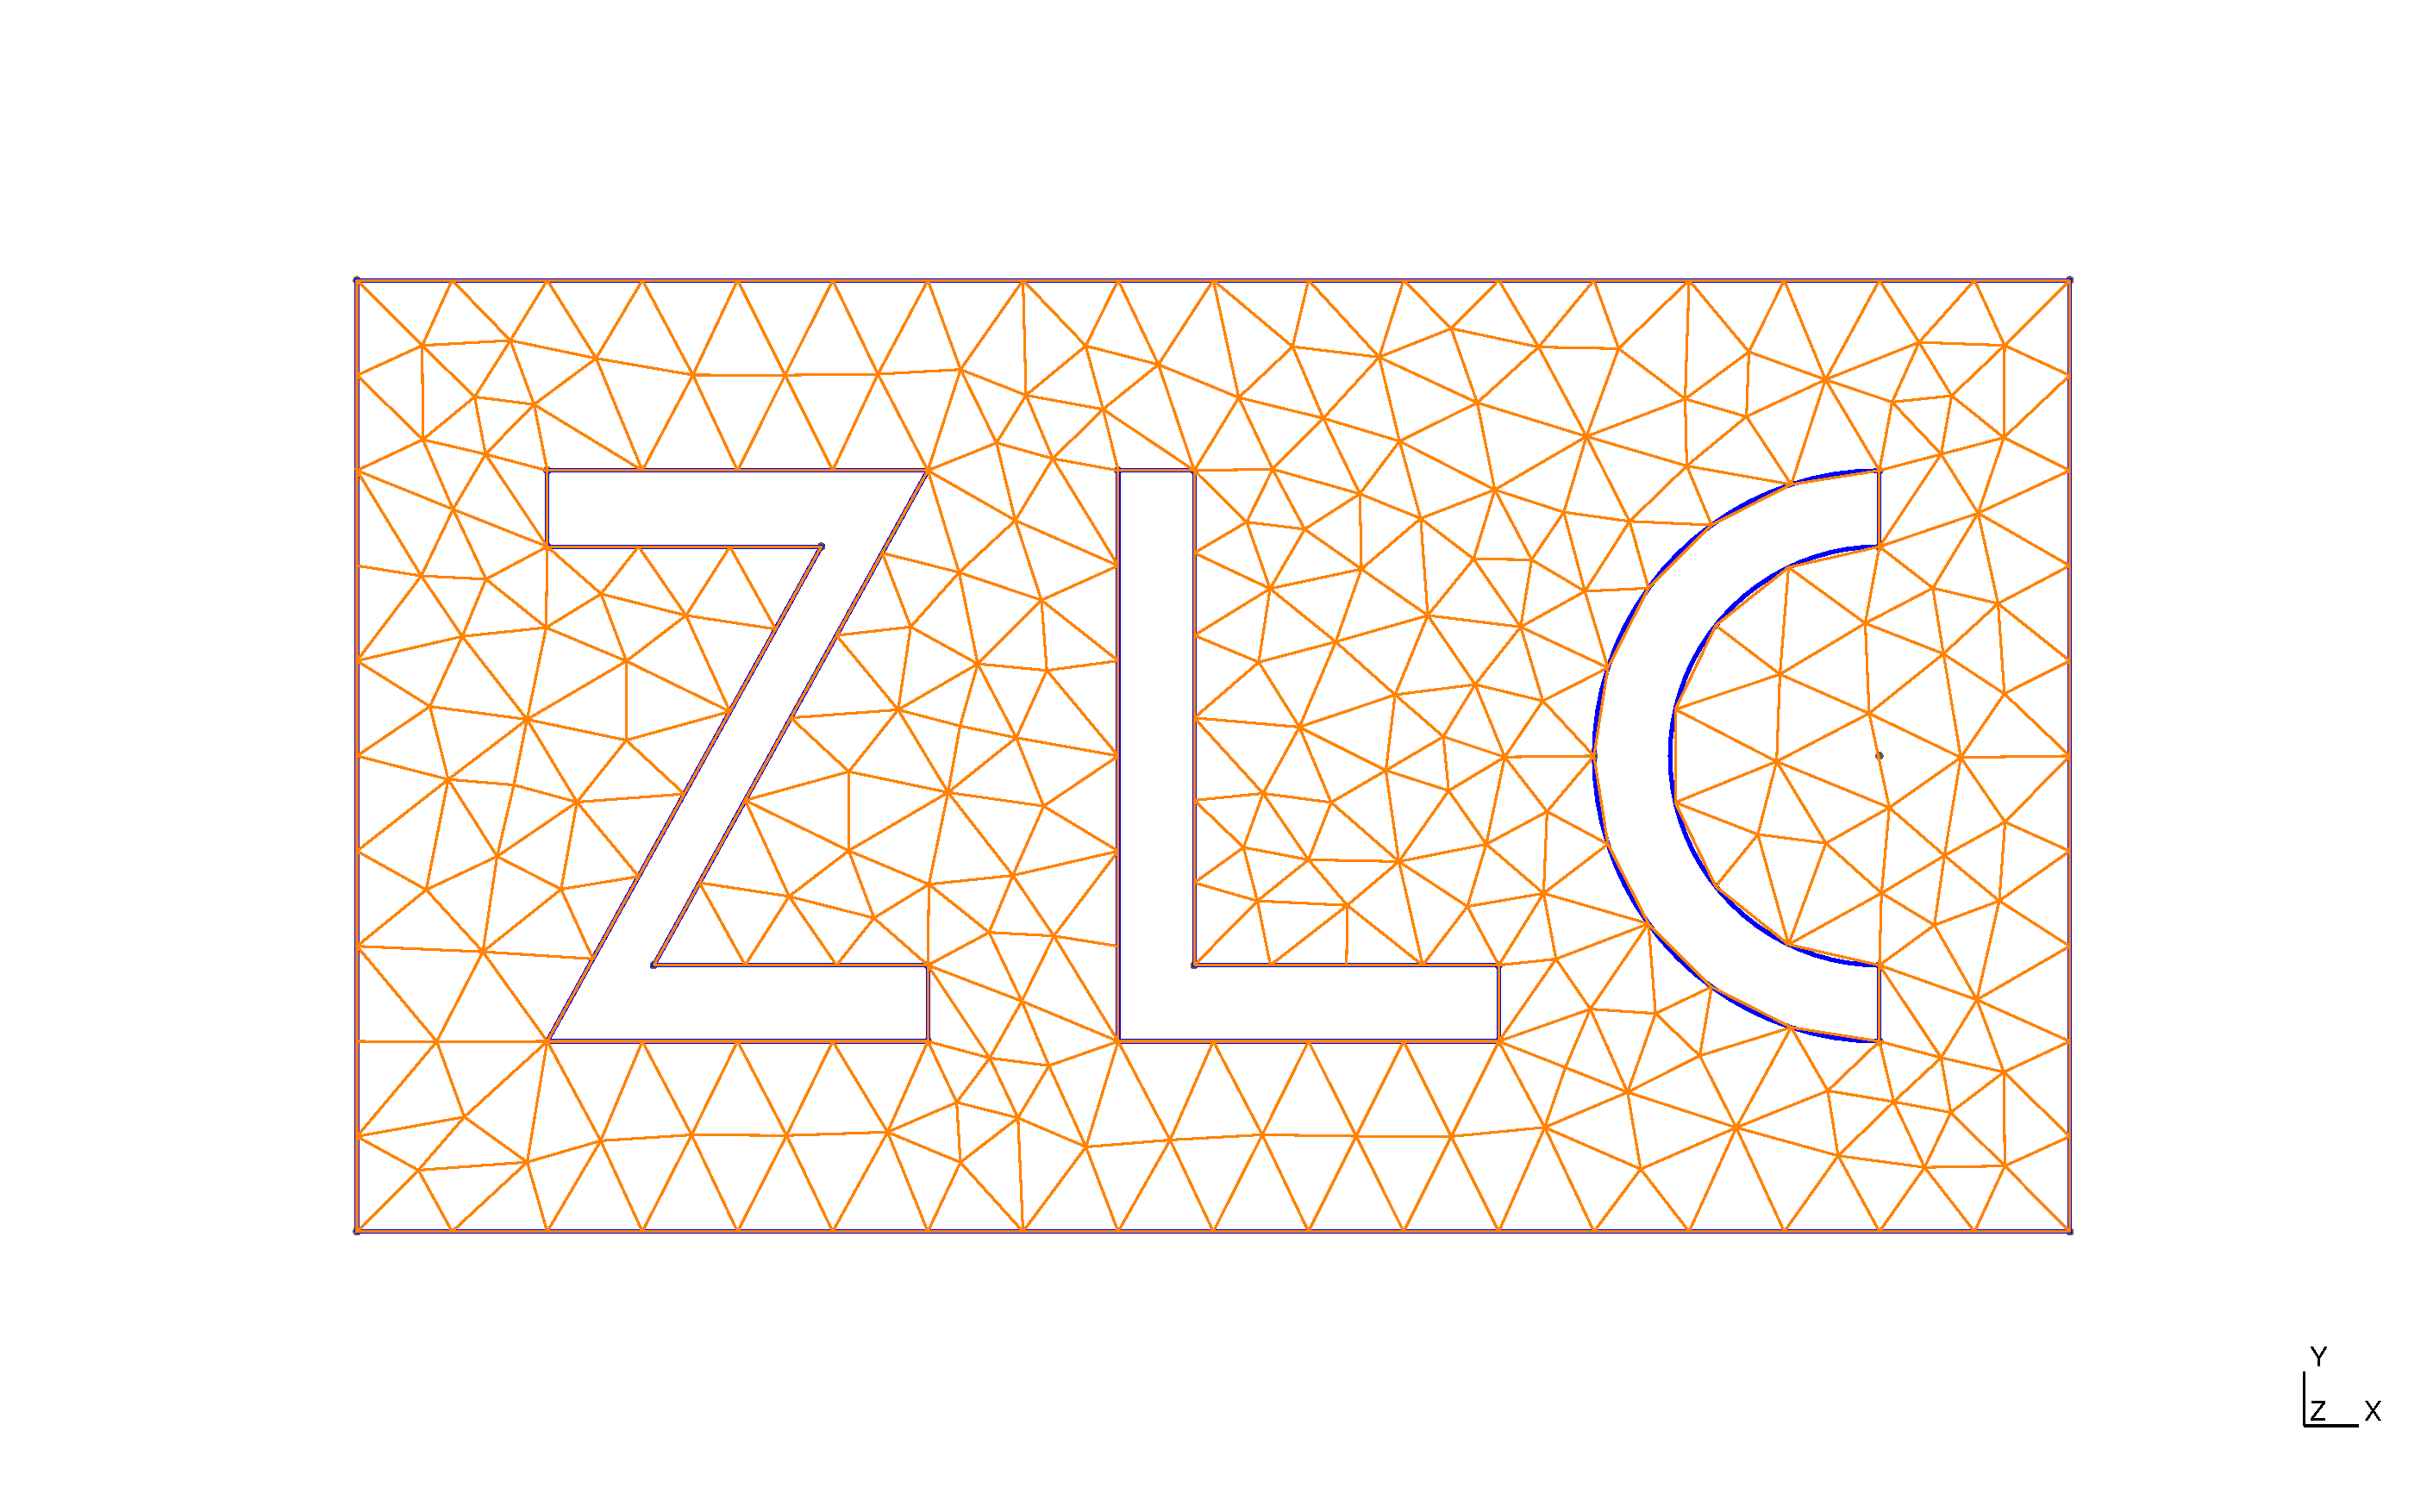
\includegraphics[width=0.9\textwidth]{zlc.eps}
	\end{center}
	\caption{简单的例子}
\end{figure}
以下是实现这个例子的geo文件代码,体现了Gmsh的基本操作。
\inputccode{zlc.geo}
\subsubsection{网格加密}
通过~\verb|RefineMesh|~命令,可以通过将当前的每个网格进行分割,从而完
成网格加密。
\subsubsection{网格密度设置}
一个简单的设置密度的形式是设置点和曲线的特征尺度
~\verb|Mesh.CharacteristicLengthFromPionts|~和
~\verb|Mesh.CharacteristicLengthFromCurvature|~。 \par
此外通过~\verb|Field|~命令,可以比较精细地设置网格密度。
\begin{itemize}
	\item ~\verb|Threshold|~可以设置网格根据和一个几何结构的距离来形成
		不同密度,其中~\verb|Attractor|~可以设置网格根据和一点或者一条
		线的距离来产生不同密度。
	\item ~\verb|Box|~可以设置网格在一个区域内部和外部的疏密程度的不同
		。
	\item ~\verb|MathEval|~可以设置网格密度为一个函数。
	\item ~\verb|Min|~可以设置网格密度为几个Field所设置的最小值。
\end{itemize}
\begin{figure}[H]
	\centering
	\subfigure[网格在一个点和一条线附近稠密]{
		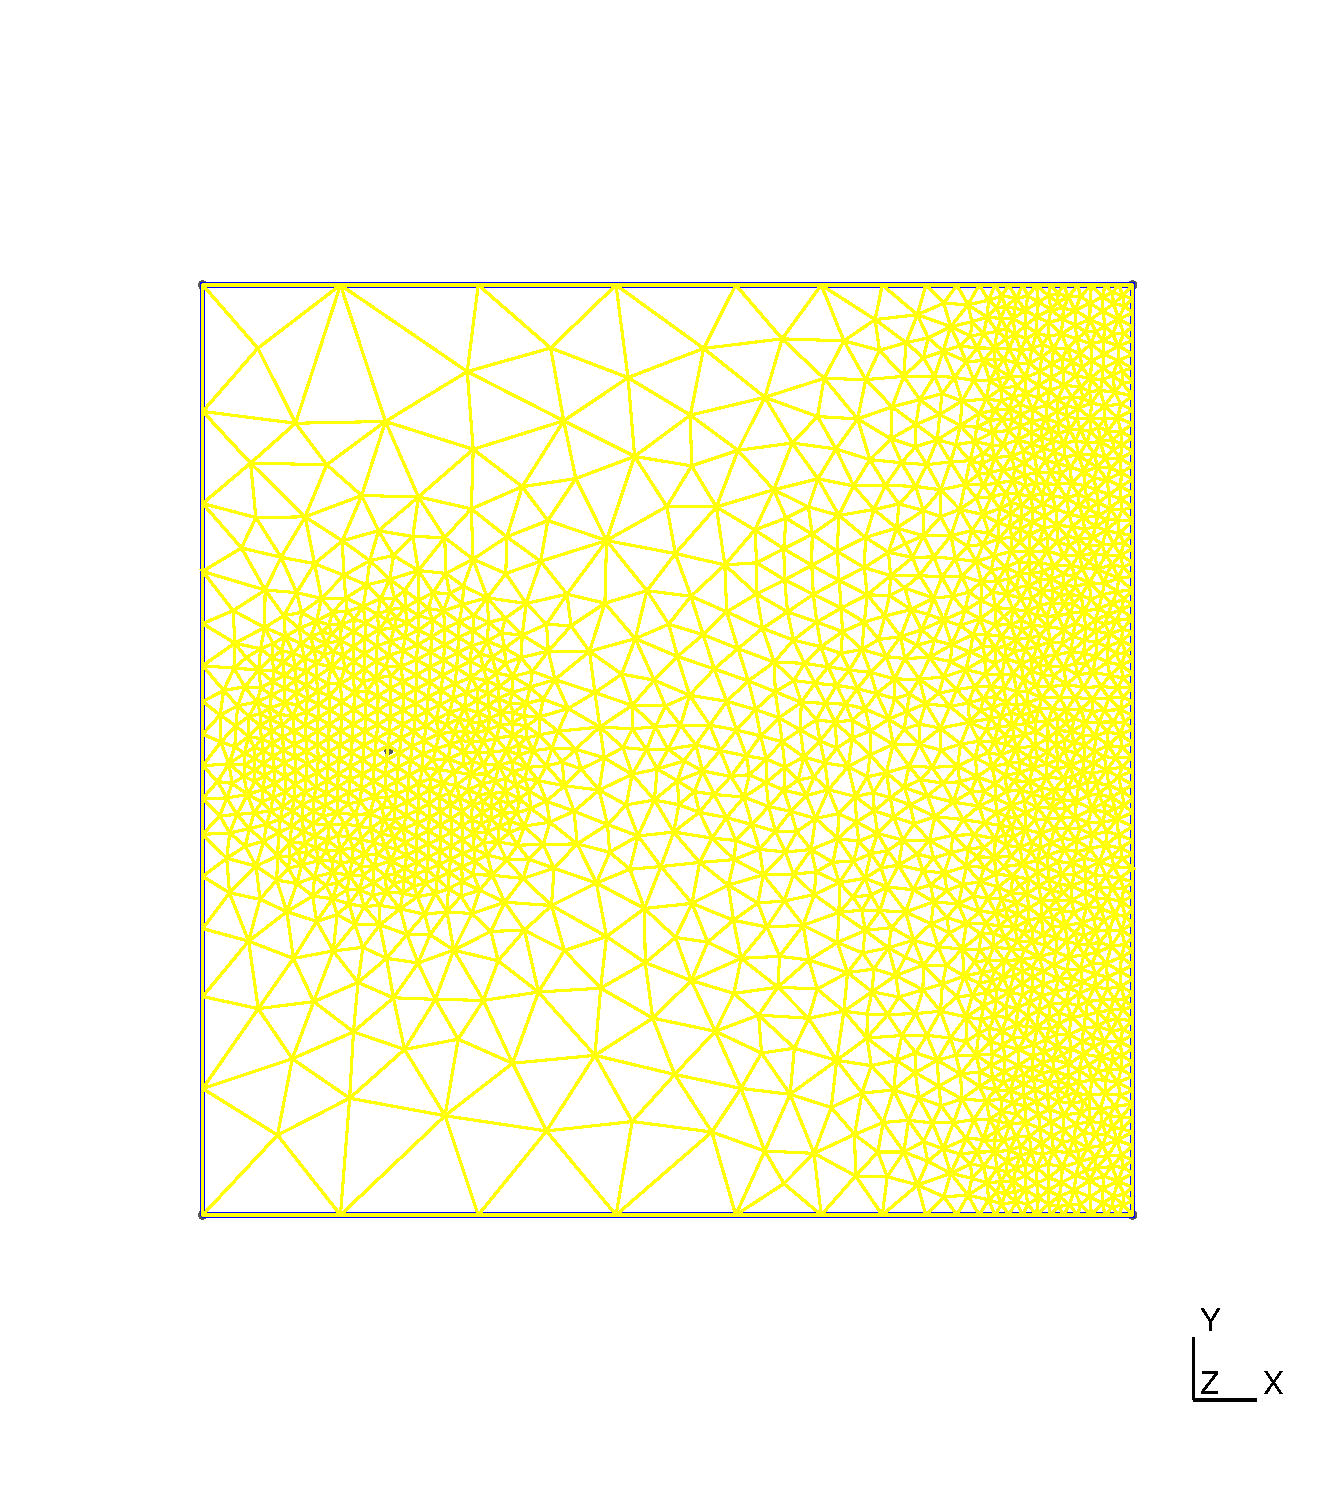
\includegraphics[width=0.4\textwidth]{field2.eps}
		}
	\subfigure[网格在抛物线附近稠密]{
		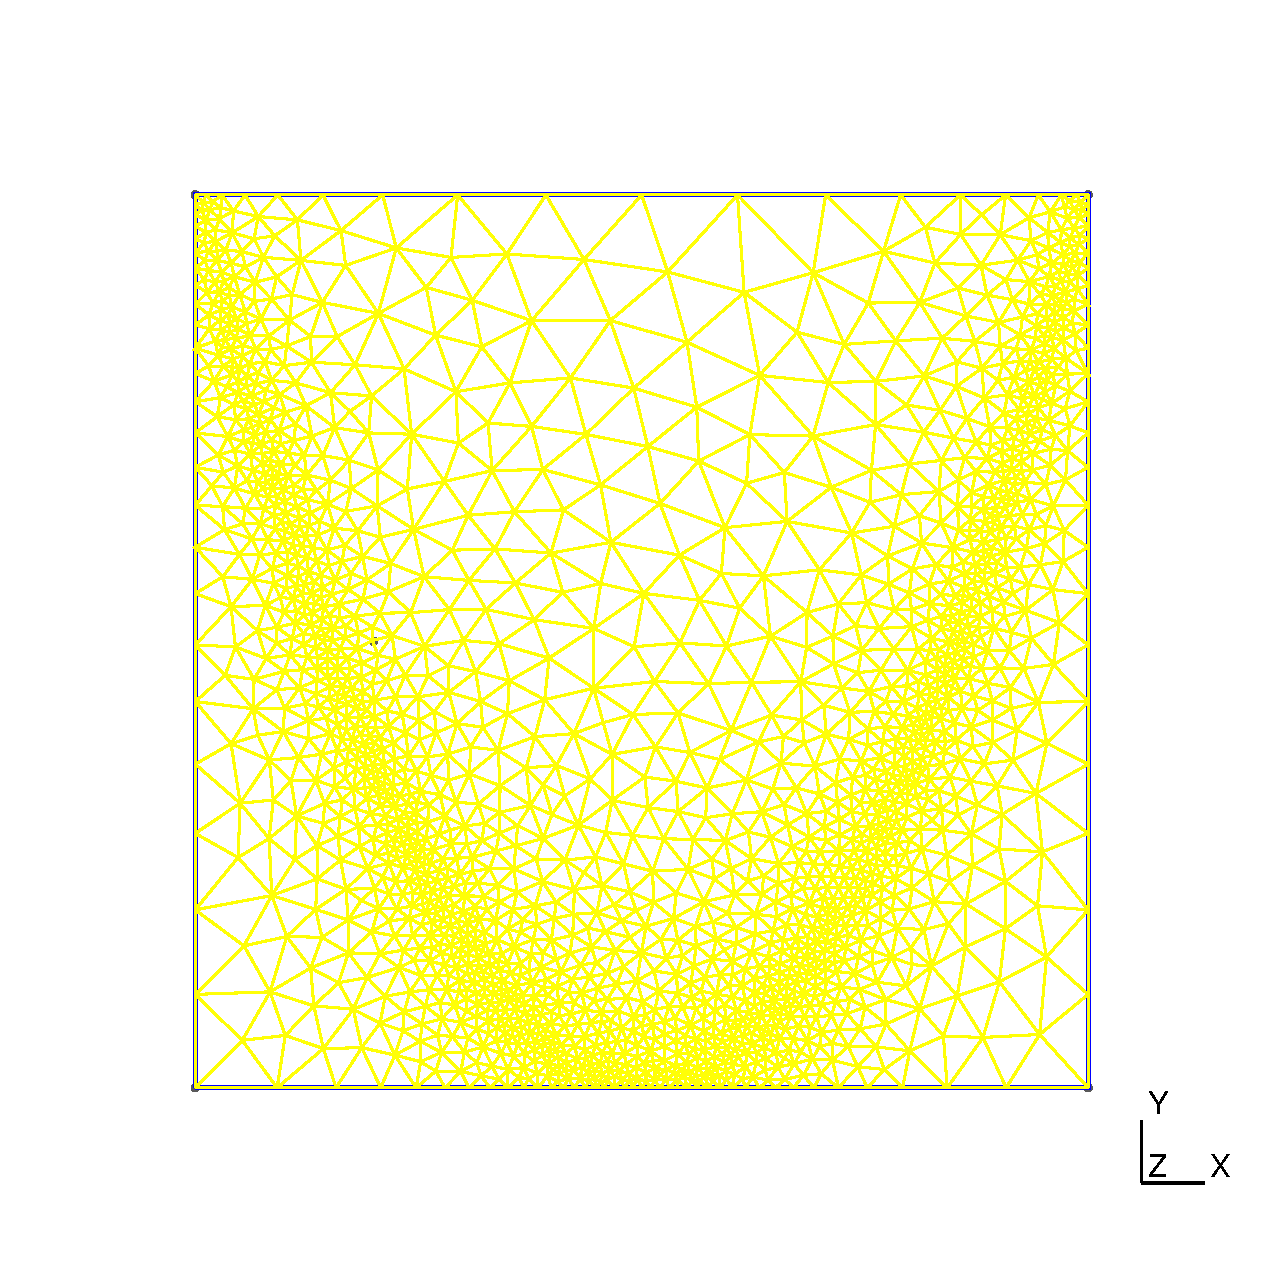
\includegraphics[width=0.4\textwidth]{charlength.eps}
		}
	\subfigure[网格在端点附近稠密]{
		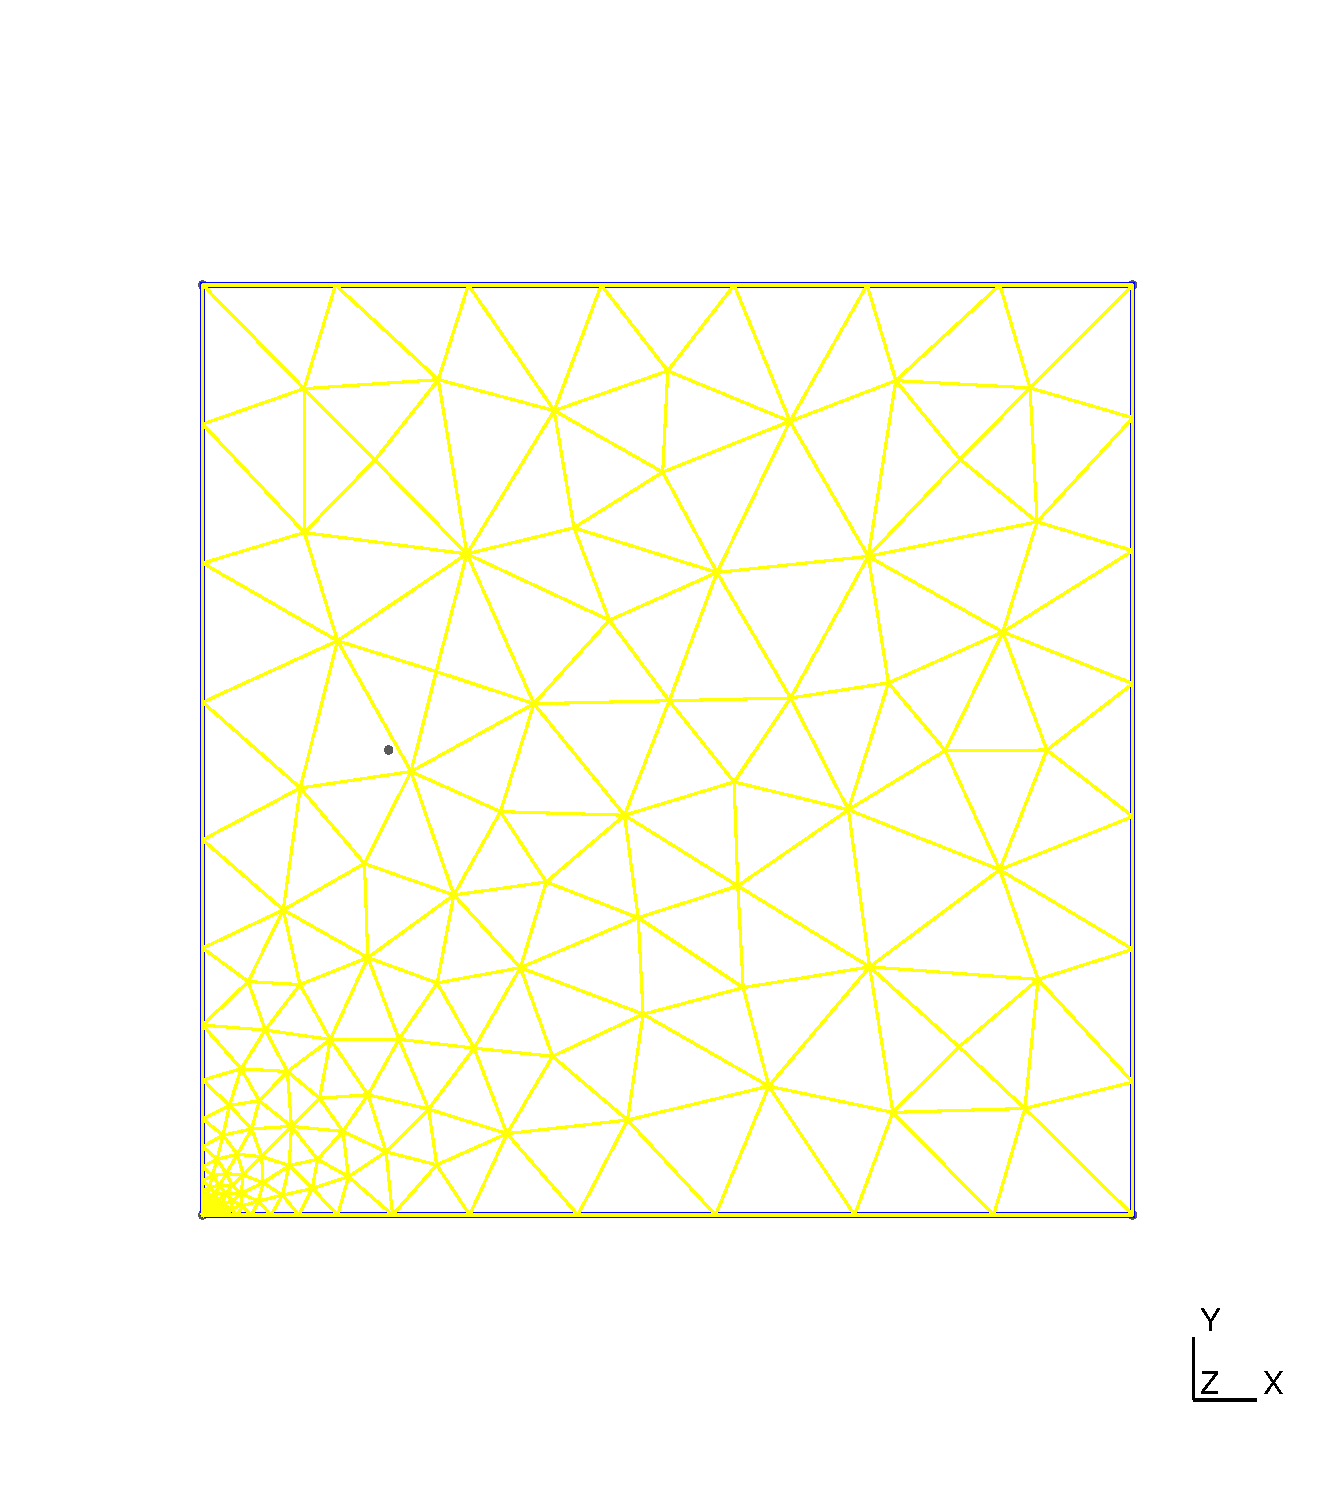
\includegraphics[width=0.4\textwidth]{field4.eps}
		}	
	\subfigure[网格在端点附近加密]{
		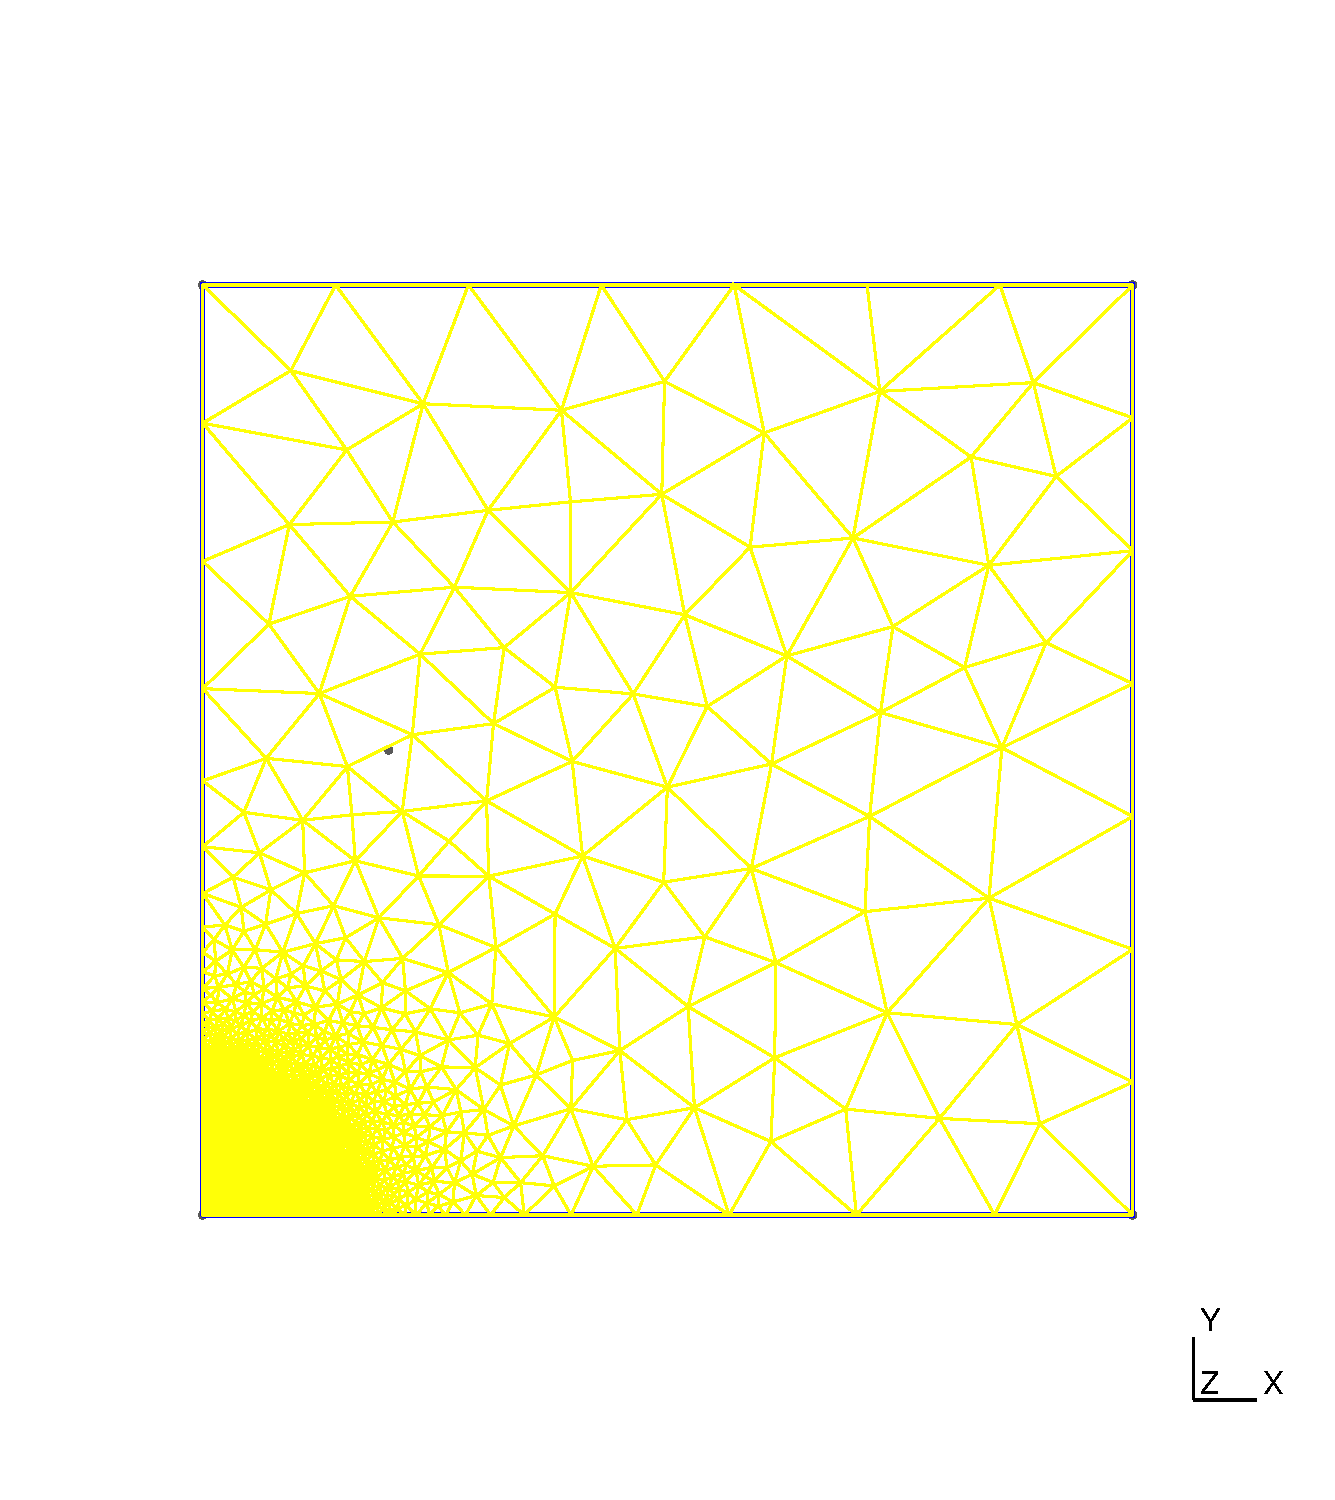
\includegraphics[width=0.4\textwidth]{field5.eps}
		}
	\subfigure[网格在区域内稠密]{
		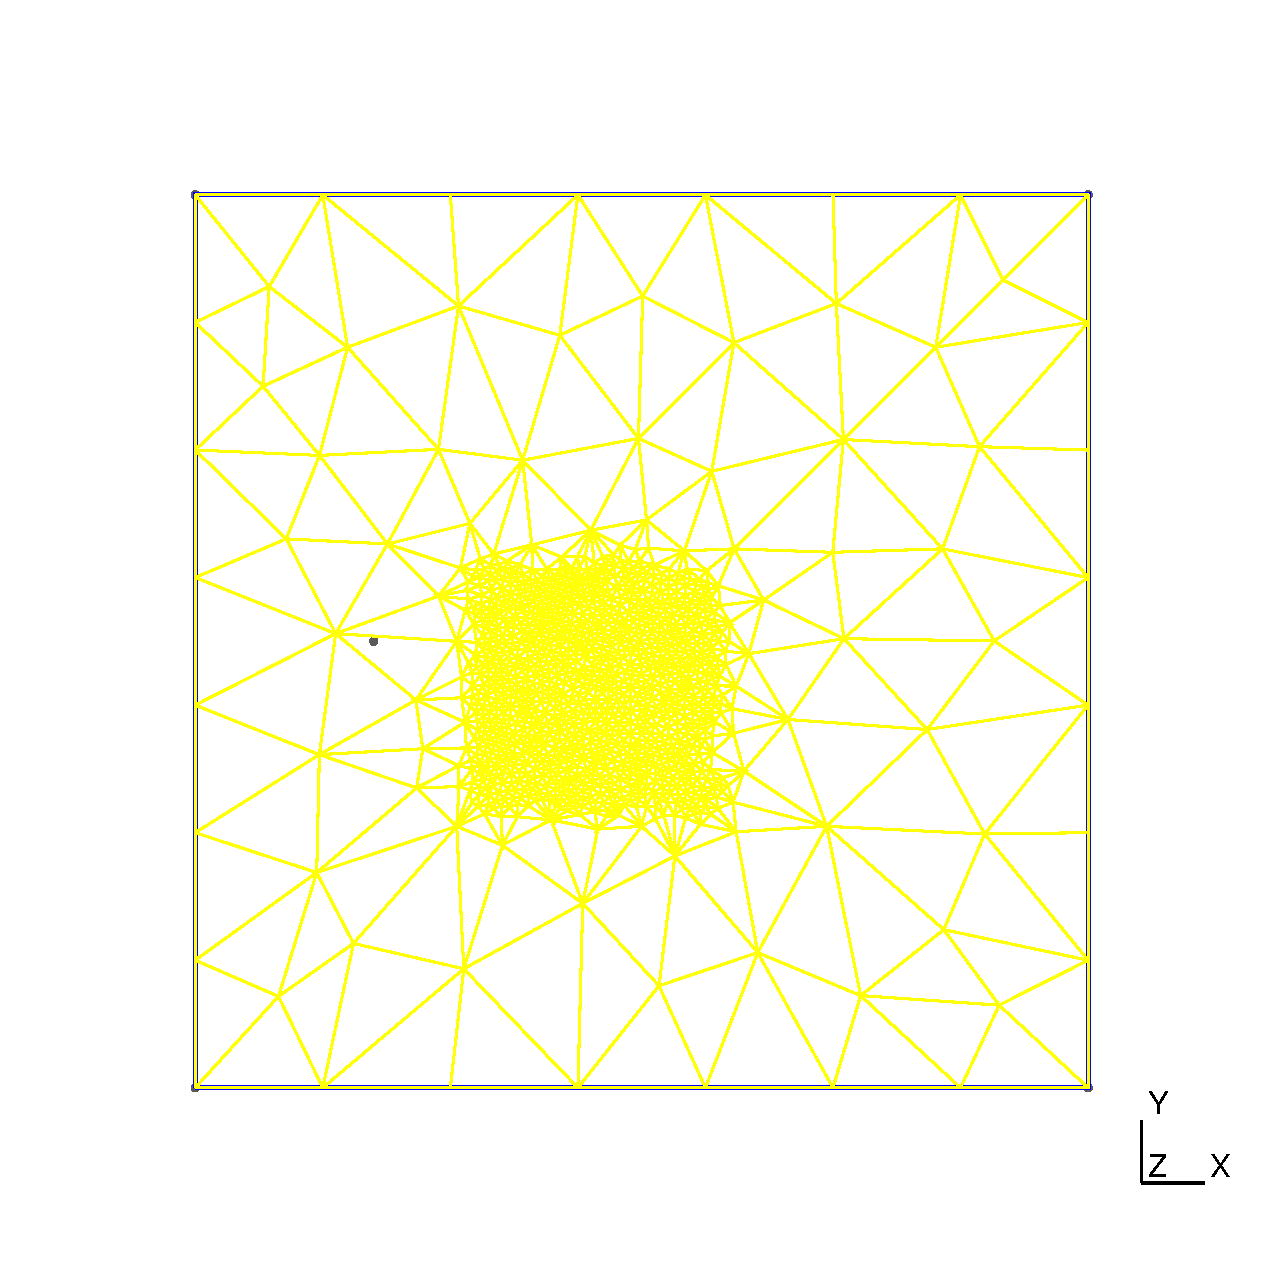
\includegraphics[width=0.4\textwidth]{box.eps}
		}
	\subfigure[网格在若干处同时稠密]{
		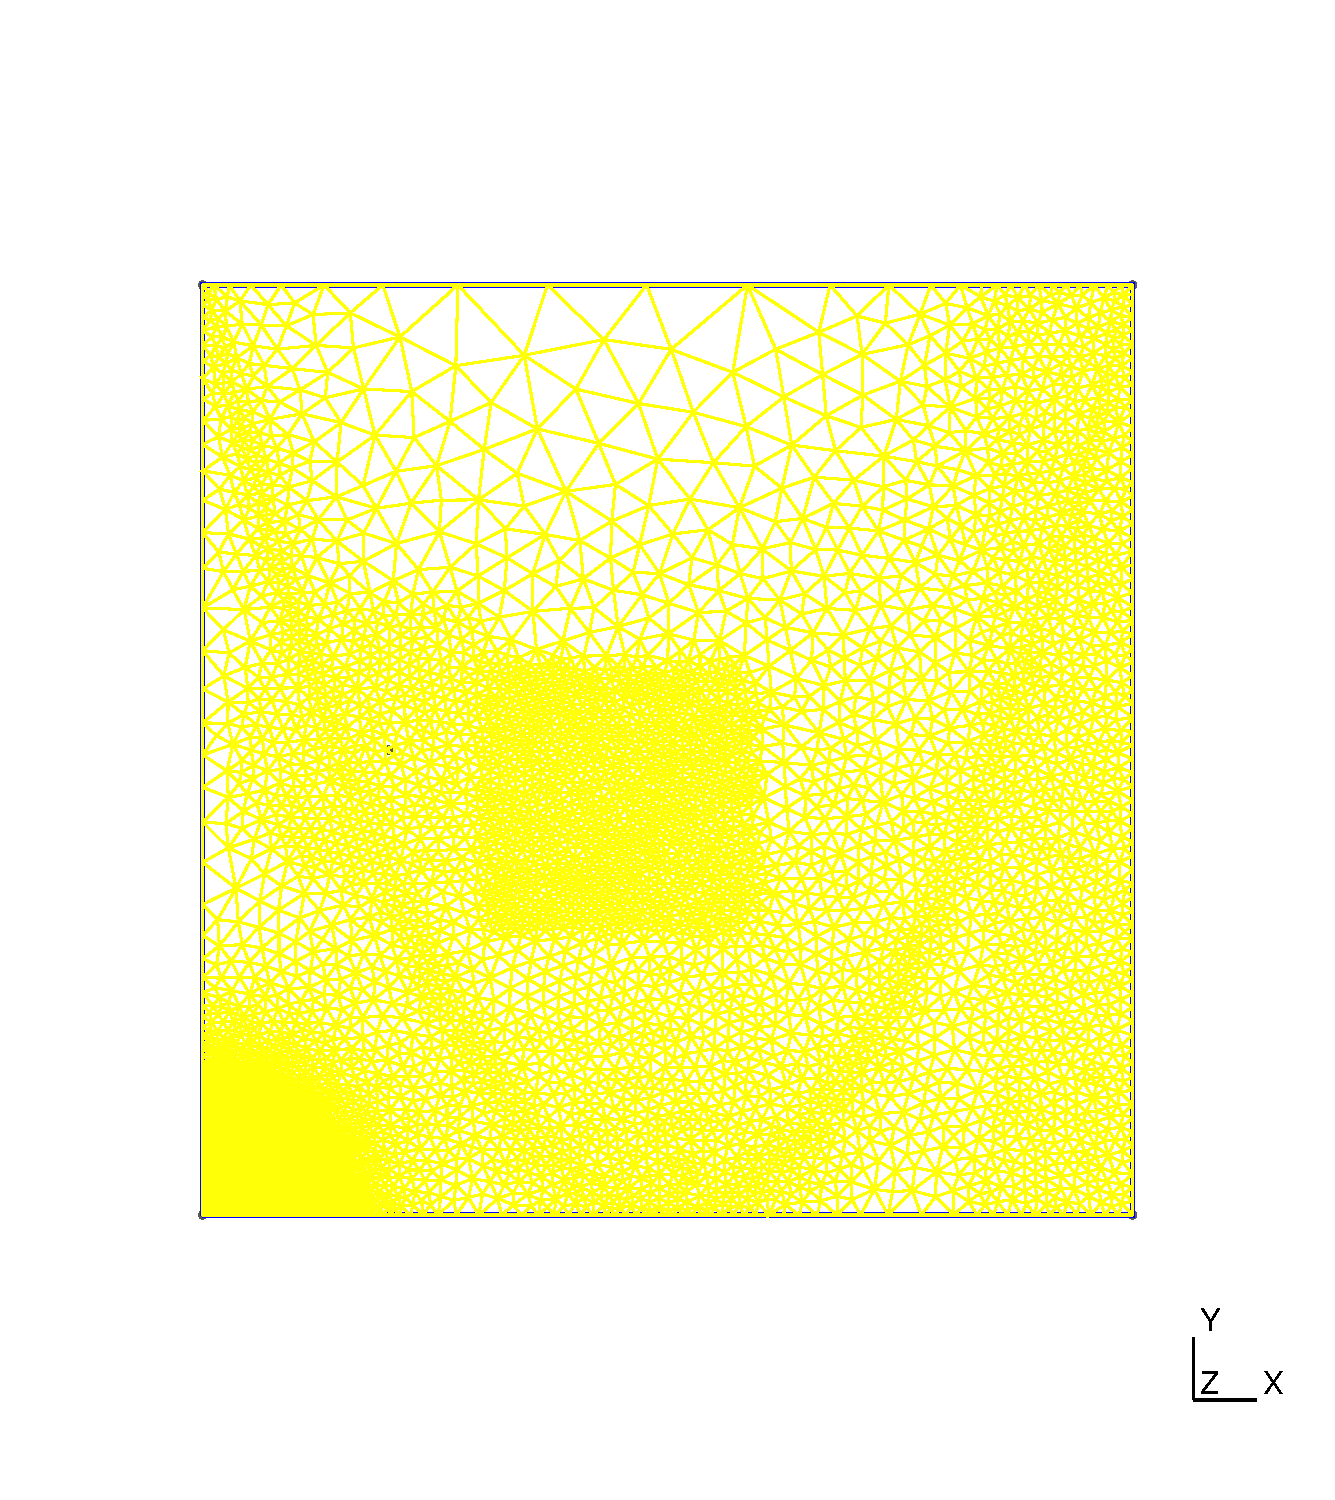
\includegraphics[width=0.4\textwidth]{field7.eps}
		}
\end{figure}
上述例子可以通过以下代码实现:
\inputccode{field.geo}
\subsubsection{二维四边形网格}
Gmsh提供了一个Recombine函数,二维情形下将三角形网格重新整合为四边形网
格。\par
\verb|Recombine Surface{expression list};| \\
其中expression list给出了所有需要整合的Surface的编号,或者采用 \par
\verb|Recombine Surface '*';| \\
来一次性整合所有Surface。

\begin{figure}[H]
	\centering
	\subfigure[三角形网格]{
		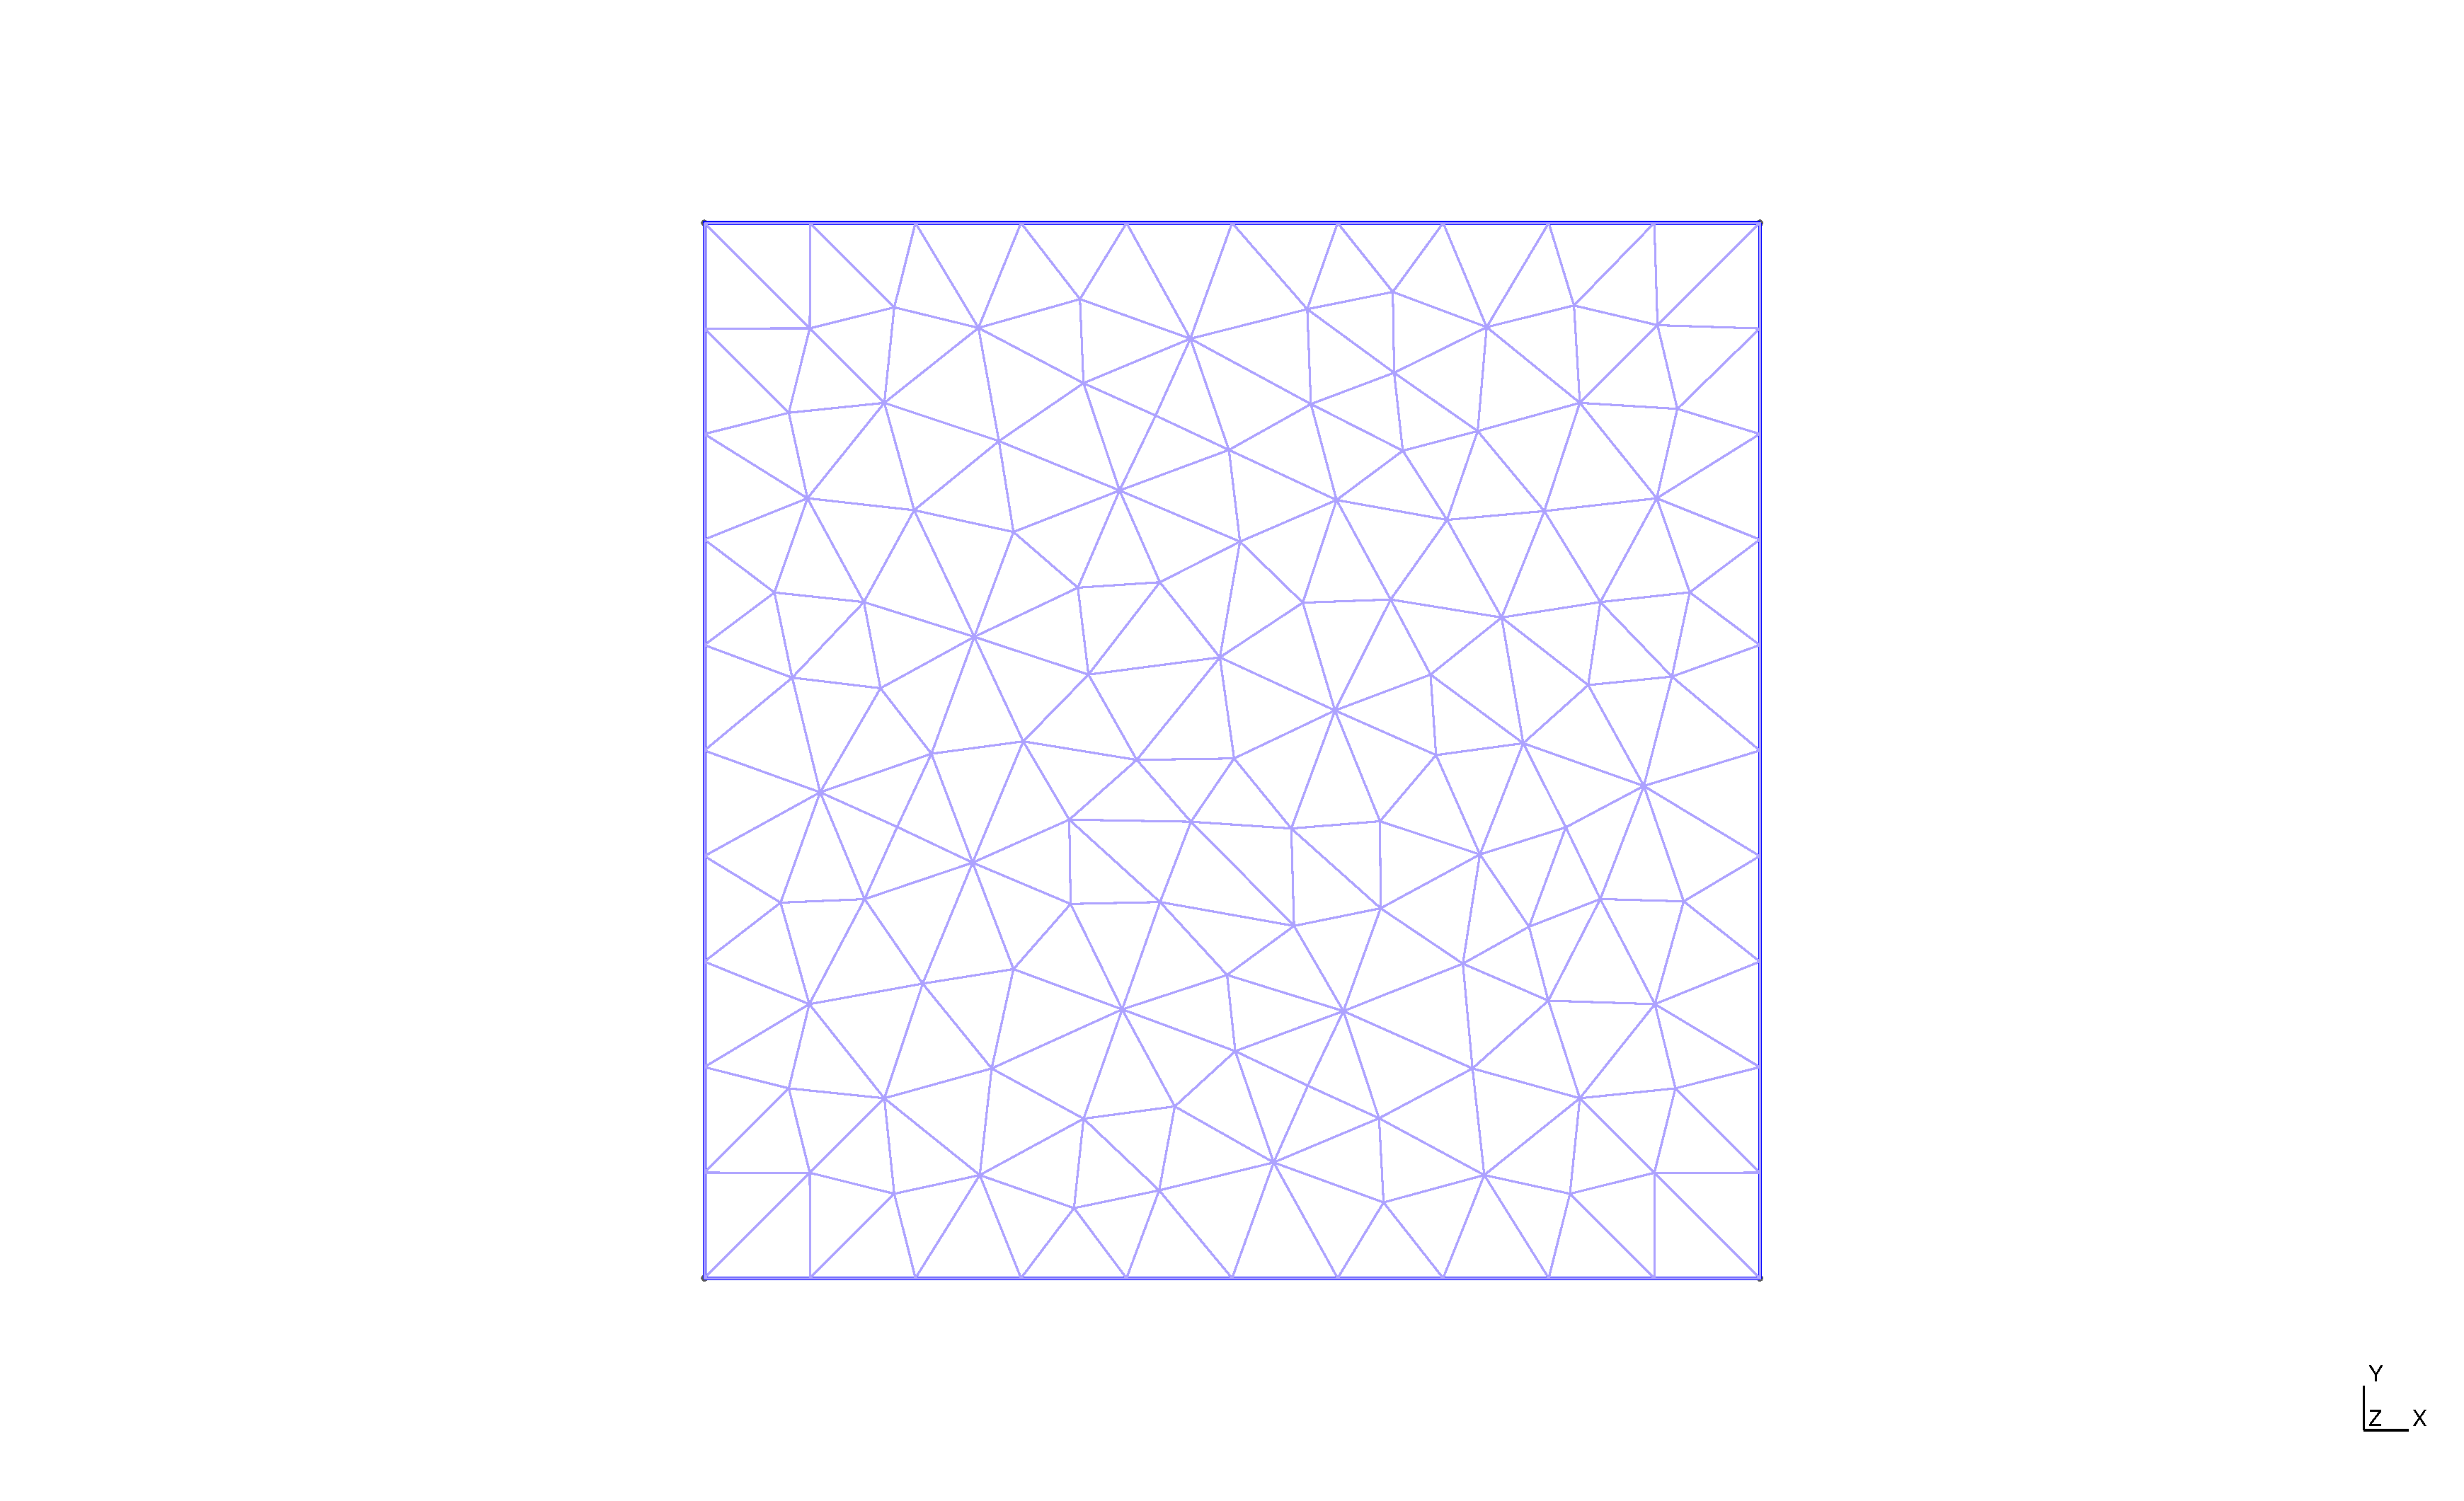
\includegraphics[width=0.45\textwidth]{triangle.eps}
		}
	\subfigure[四边形网格]{
		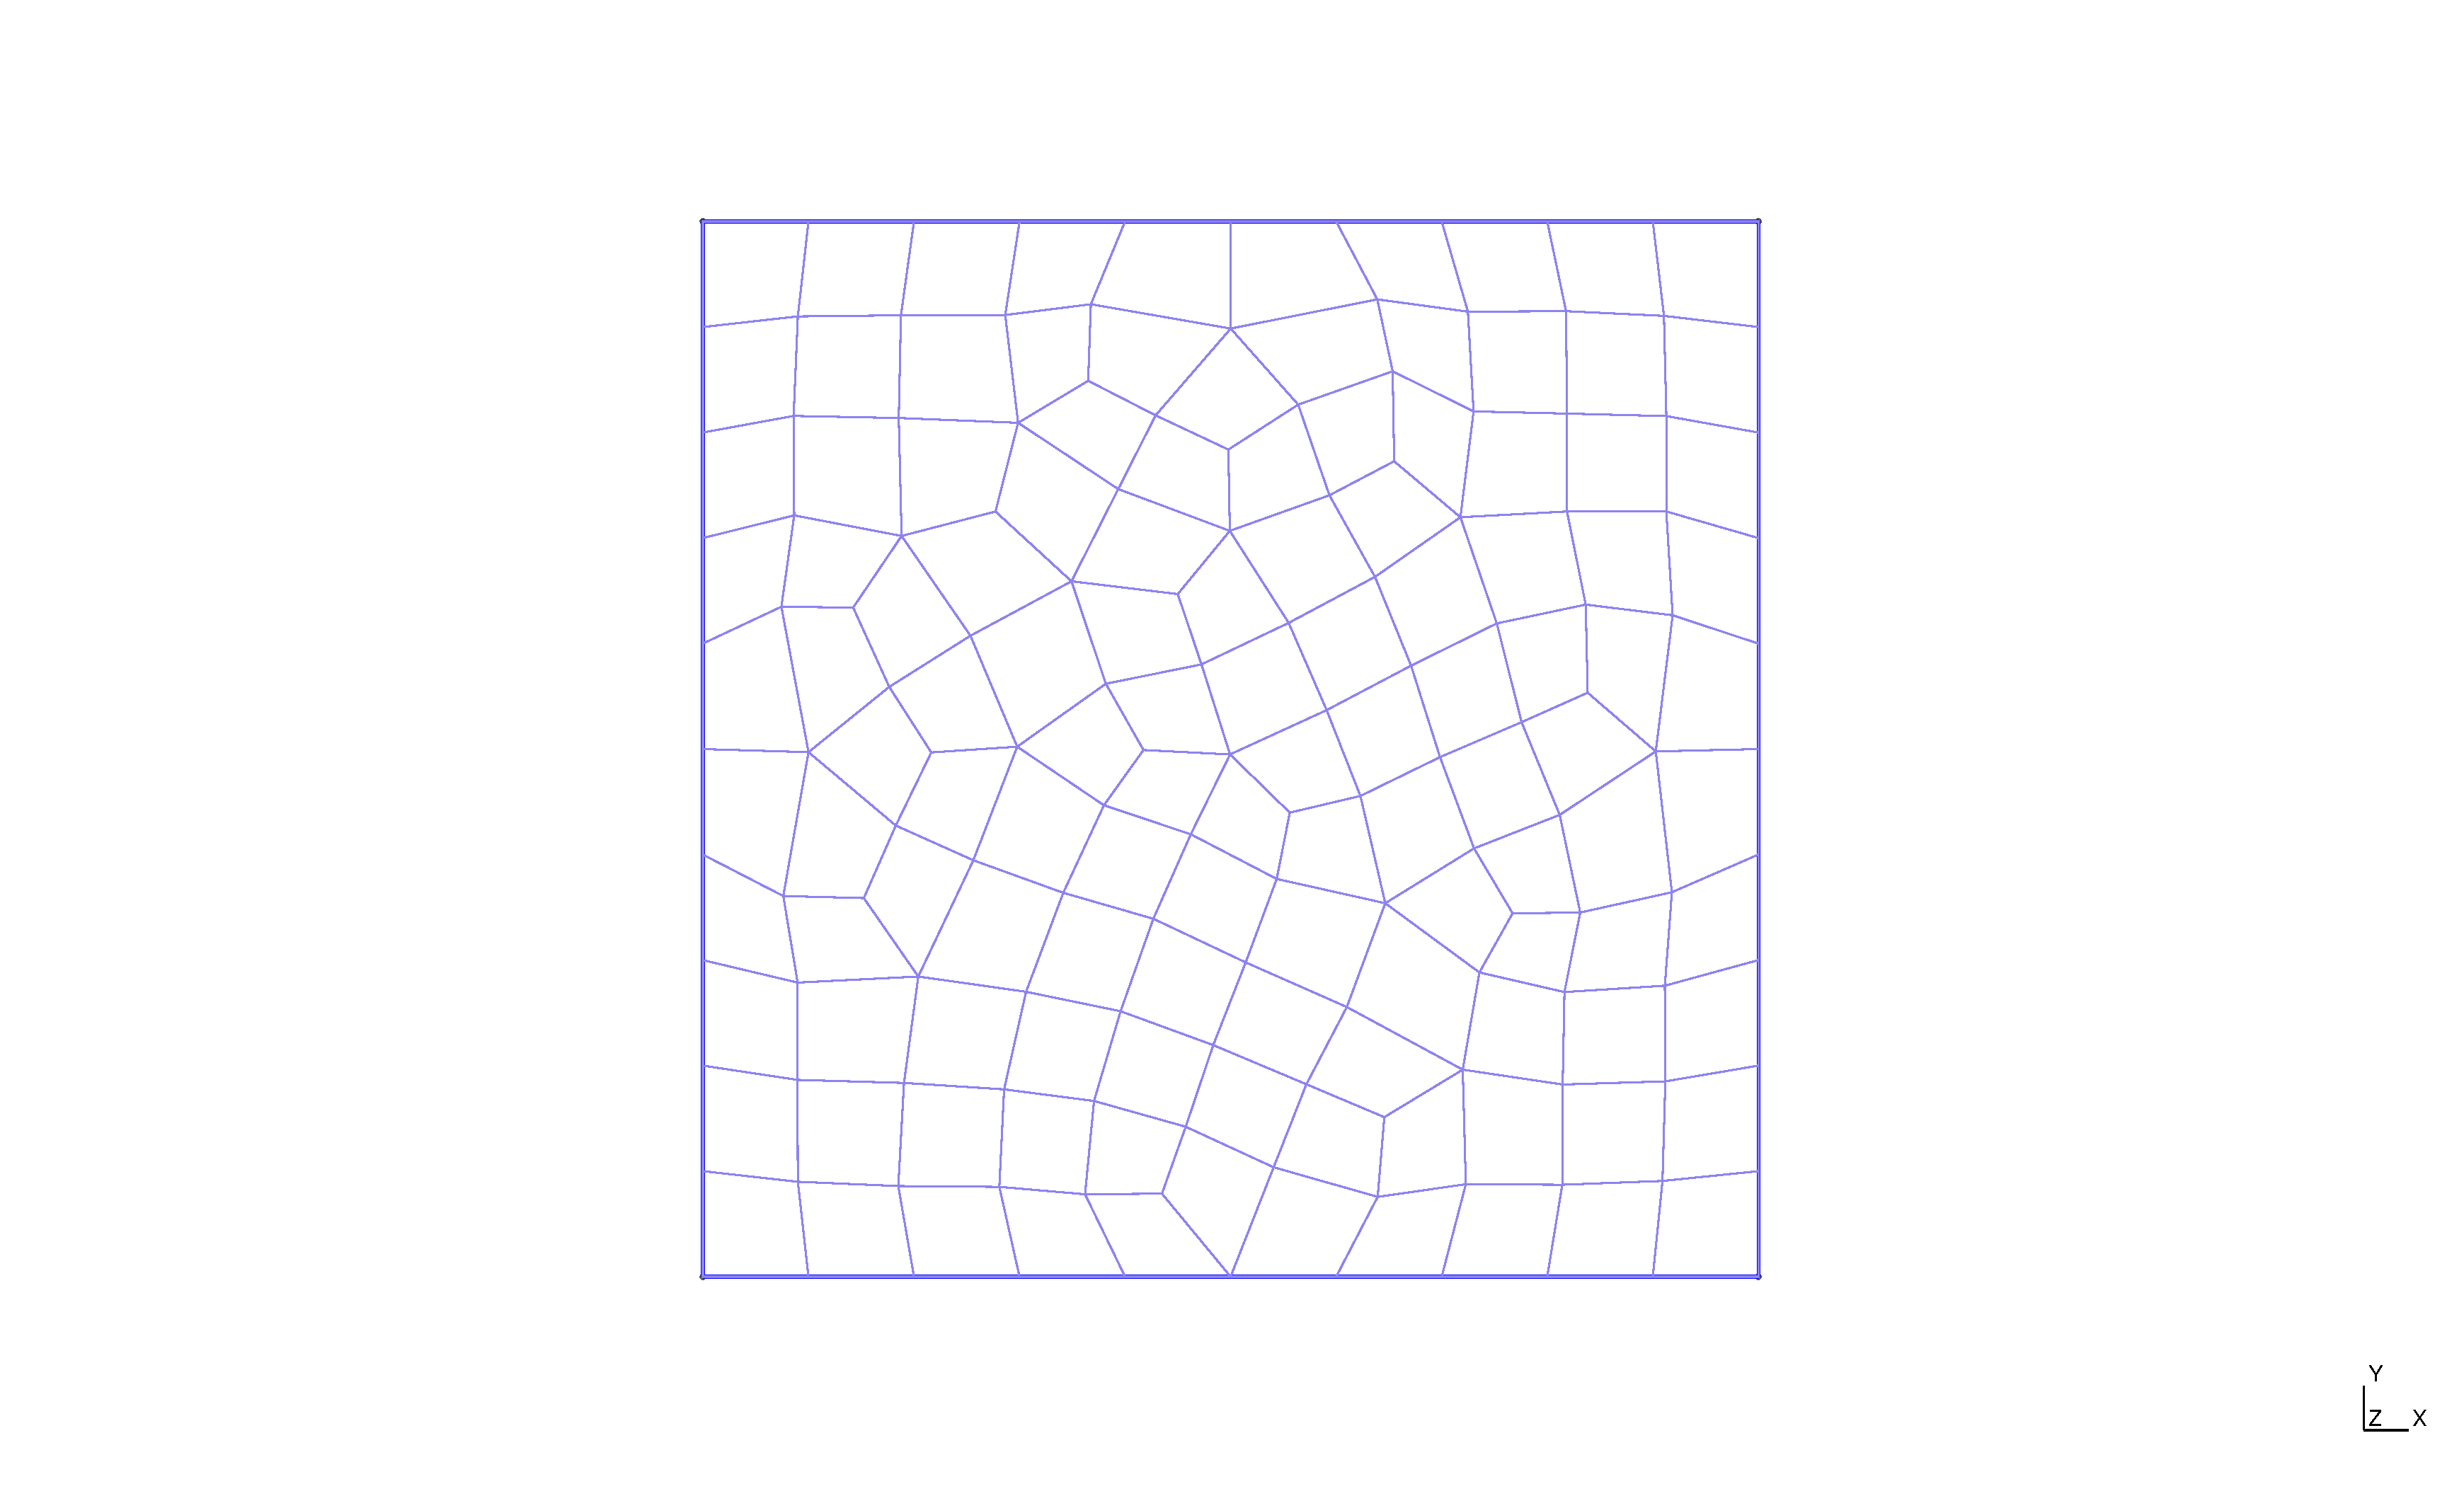
\includegraphics[width=0.45\textwidth]{quadrangle.eps}
		}
\end{figure}


\subsubsection{二维结构四边形网格}
要生成二维结构四边形网格,可以采用Extrude来完成。\par
\verb|Extrude { expression list} {extrude list layers} |\\
其中expression list给出了所有要被Extrude的几何体。而extrude list
layers 可以加入一些参数来决定生成网格的层数以及是否进行整合。\par
例如\par
	\verb|Extrude { 0,0.1,0 } {  Line{1};Layers{5}; };| \\
	可以生成左图,其中Layers\{5\}表示在移动方向(此处为数值方向)
	上生成5个层次。\par
	\verb|Extrude { 0,0.1,0 } {  Line{1};Layers{5}; Recombine; };| \\
	可以生成右图,其中Recombine表示要进行整合,整合结果为矩形网格。\par
\begin{figure}[H]
	\centering
	\subfigure[结构三角形网格]{
	
		\includegraphics[width=0.45\textwidth]{structtriangle.eps}
		}
	\subfigure[结构四边形网格]{
		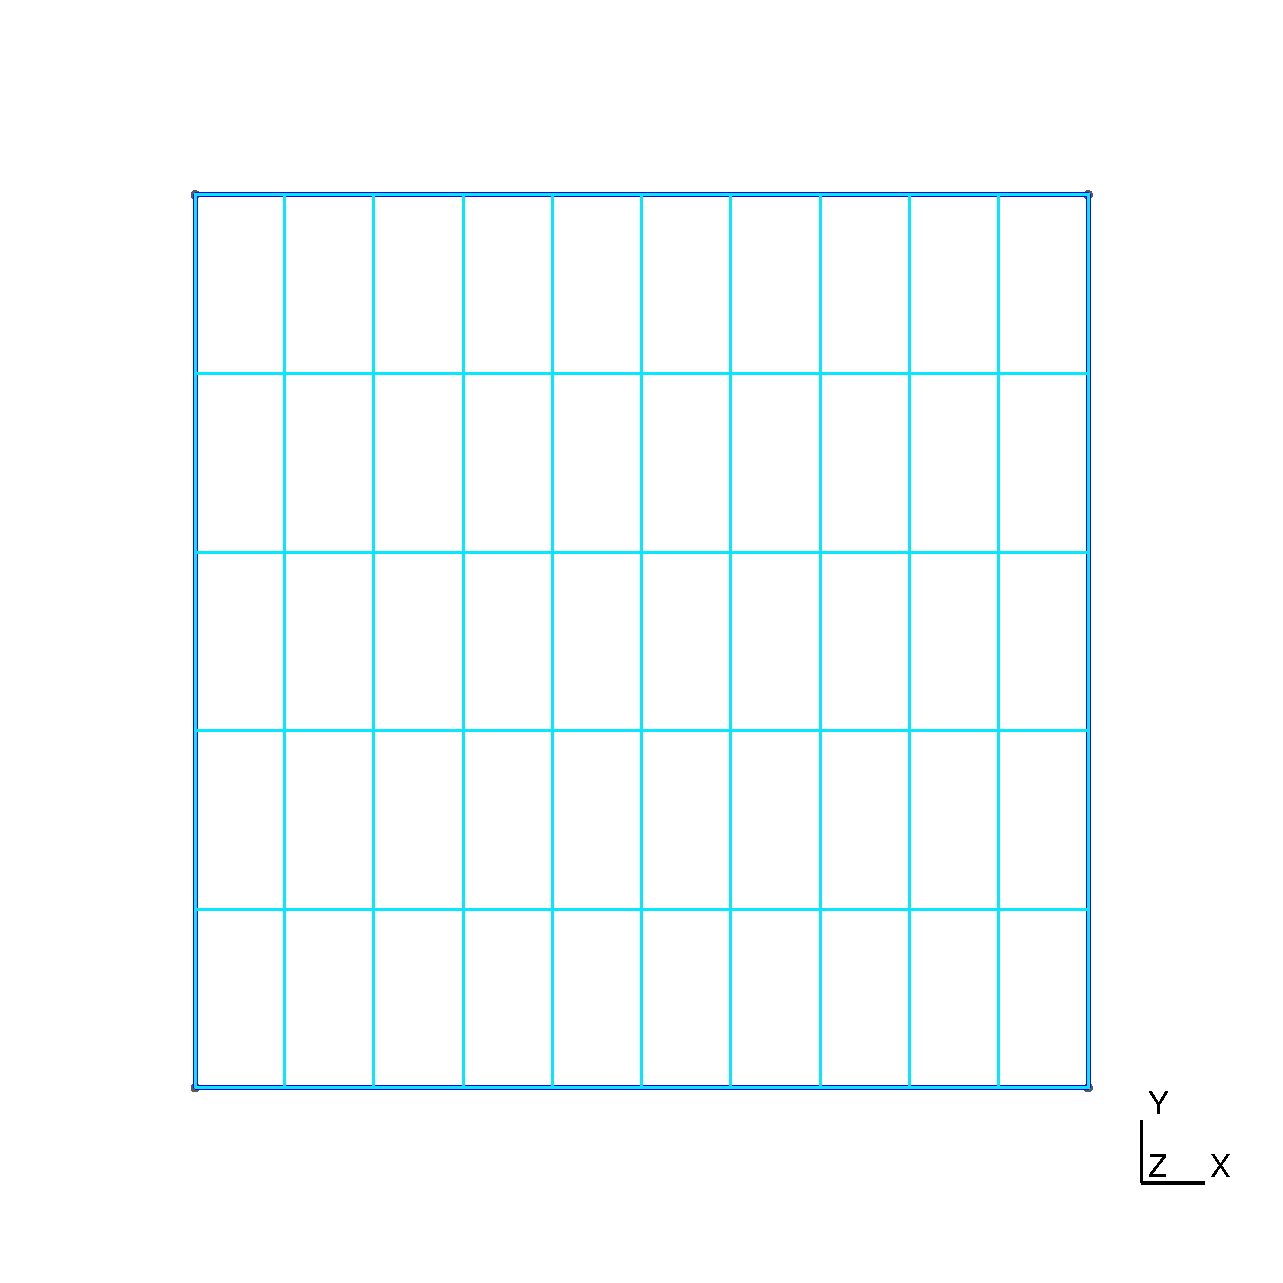
\includegraphics[width=0.45\textwidth]{structquadrangle.eps}
		}
\end{figure}
\subsection{三维网格}
\subsubsection{三维四面体网格}
在对区域进行三维的网格剖分时,Gmsh默认按照无结构四面体网格剖分,因此只
需要\par
~\verb|gmsh test.geo -3|~ \\
就可以对test.geo进行三维的四面体网格剖分。
\subsubsection{三维结构网格}
对于三维区域,若要生成除了四面体之外的网格,需要采用结构网格的形式,即
采用~\verb|Extrude|~ 命令。以下我们给出一个简单的生成长方体网格的代码
。
\inputccode{cuboid.geo}
\begin{figure}[H]
	\centering
	\subfigure[三维四面体网格]{
		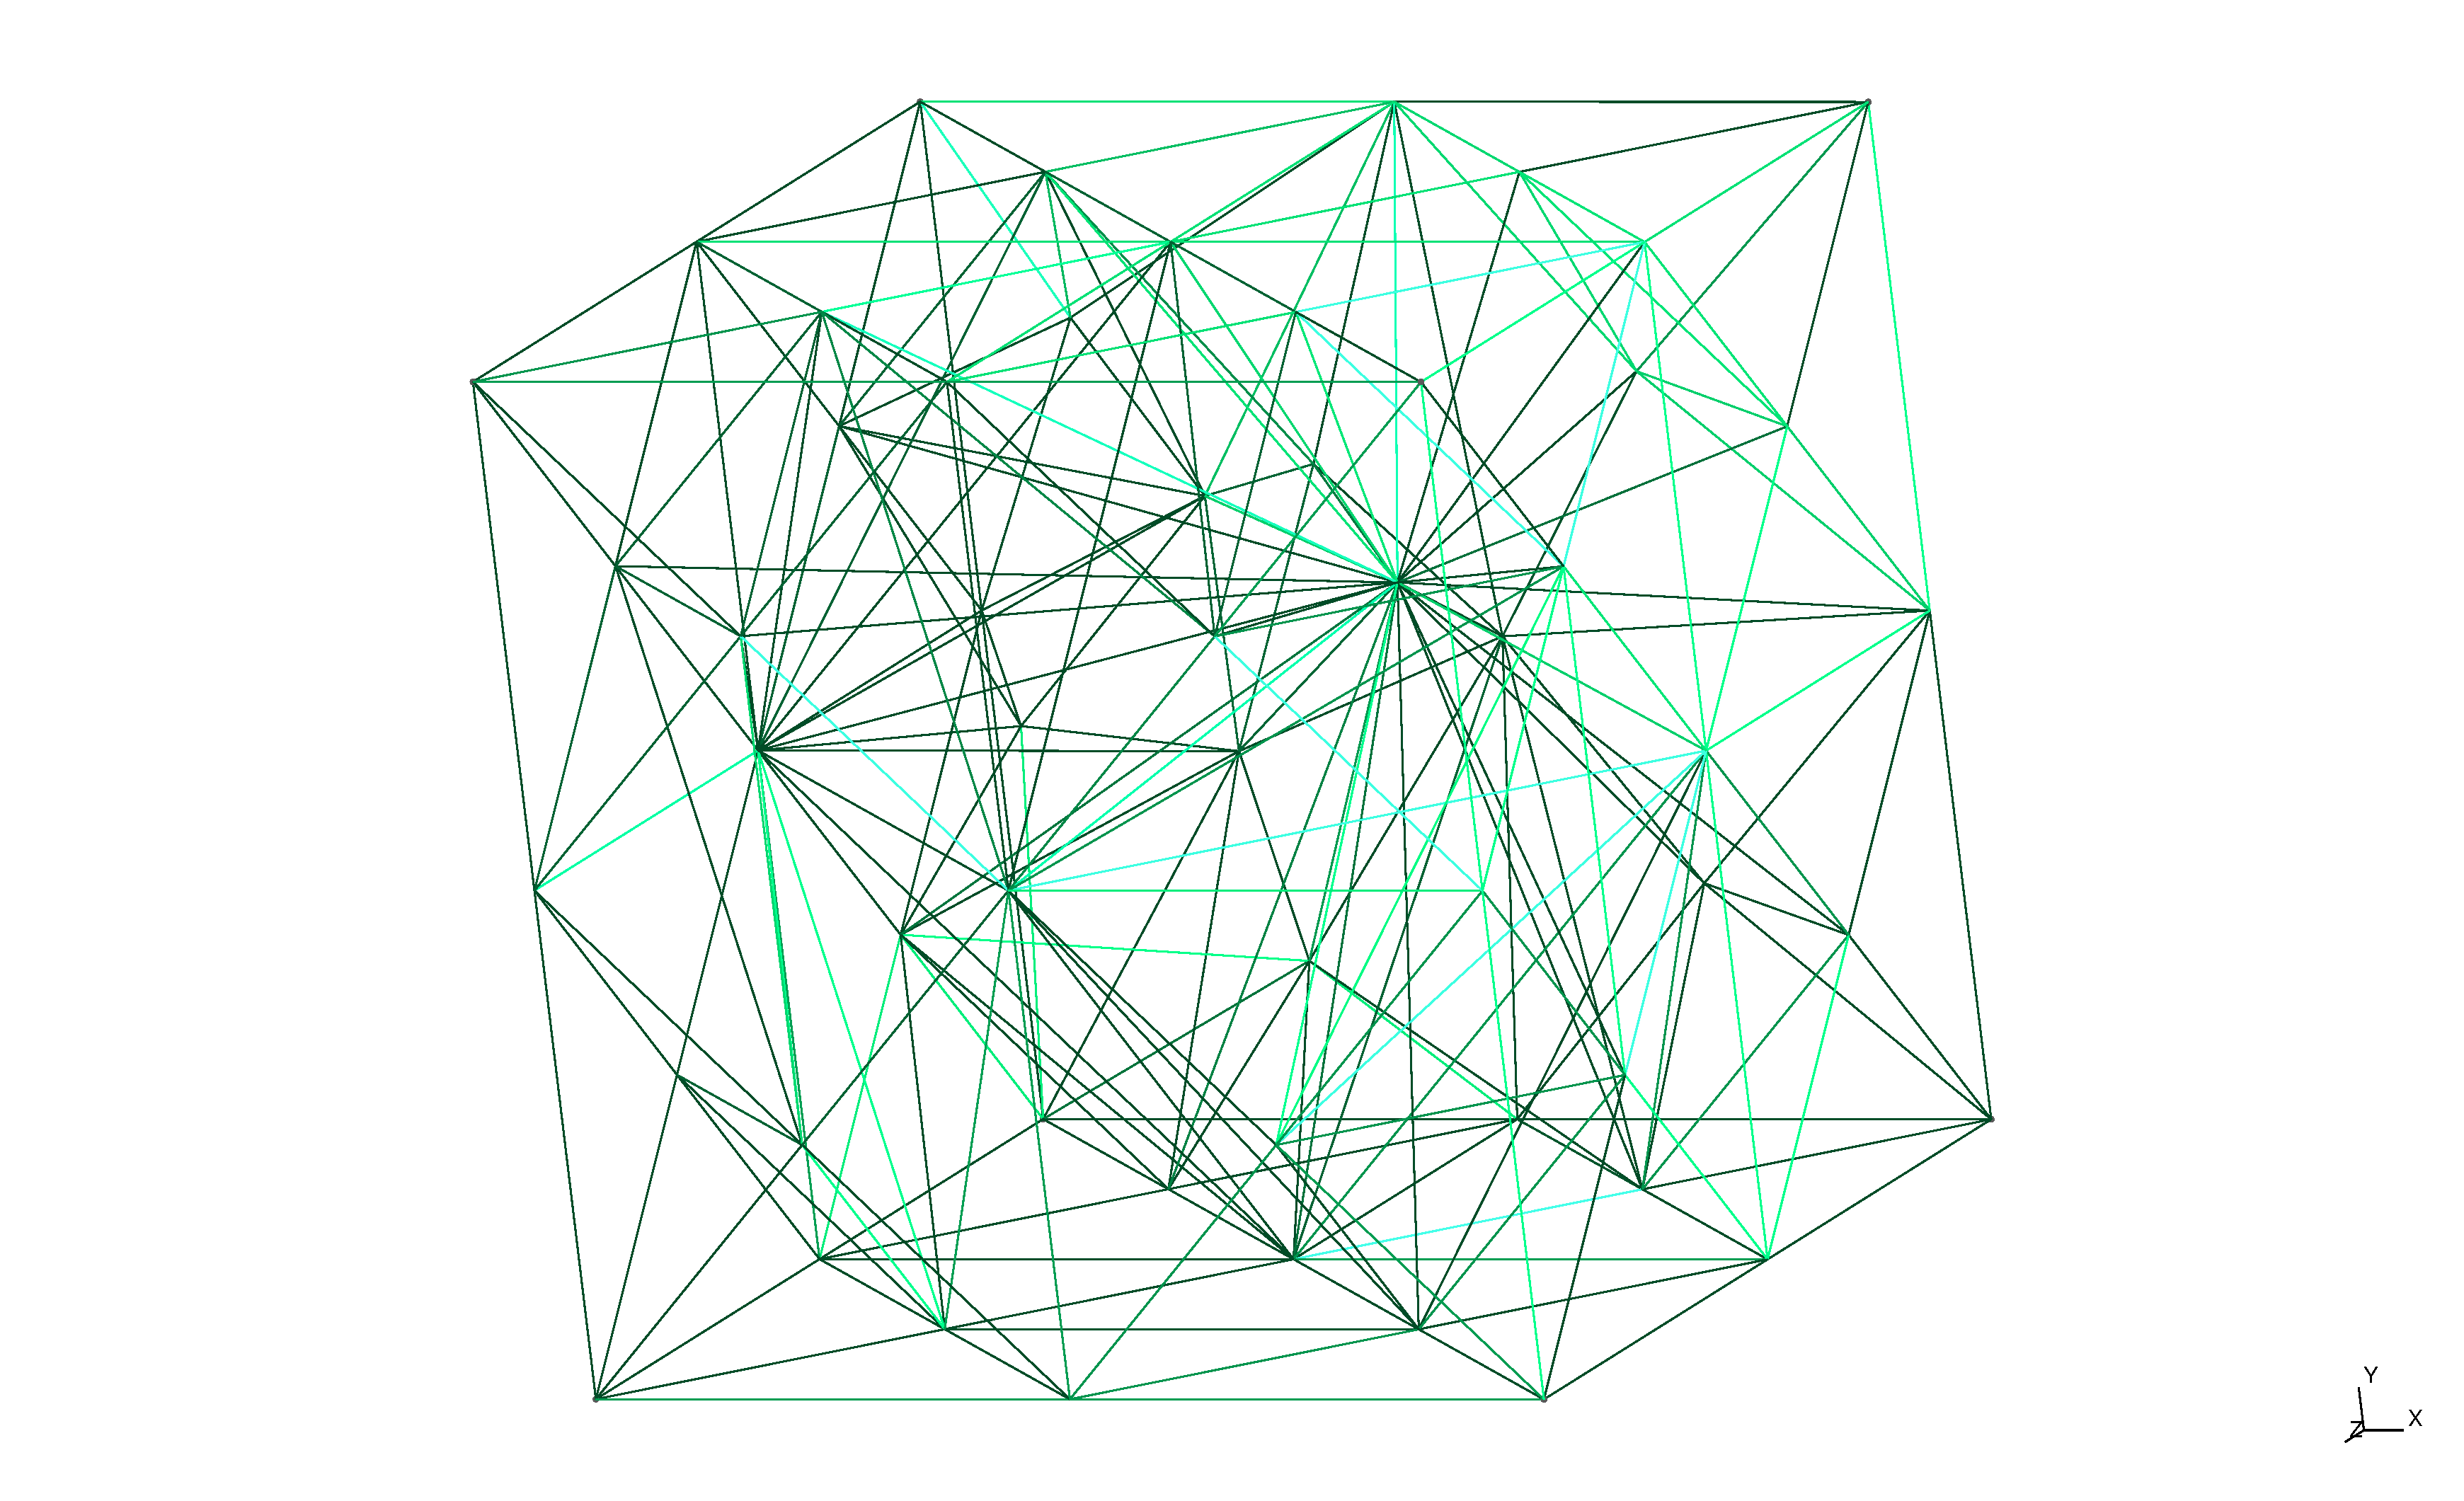
\includegraphics[width=0.45\textwidth]{tetra.eps}
		}
	\subfigure[三维长方体网格]{
		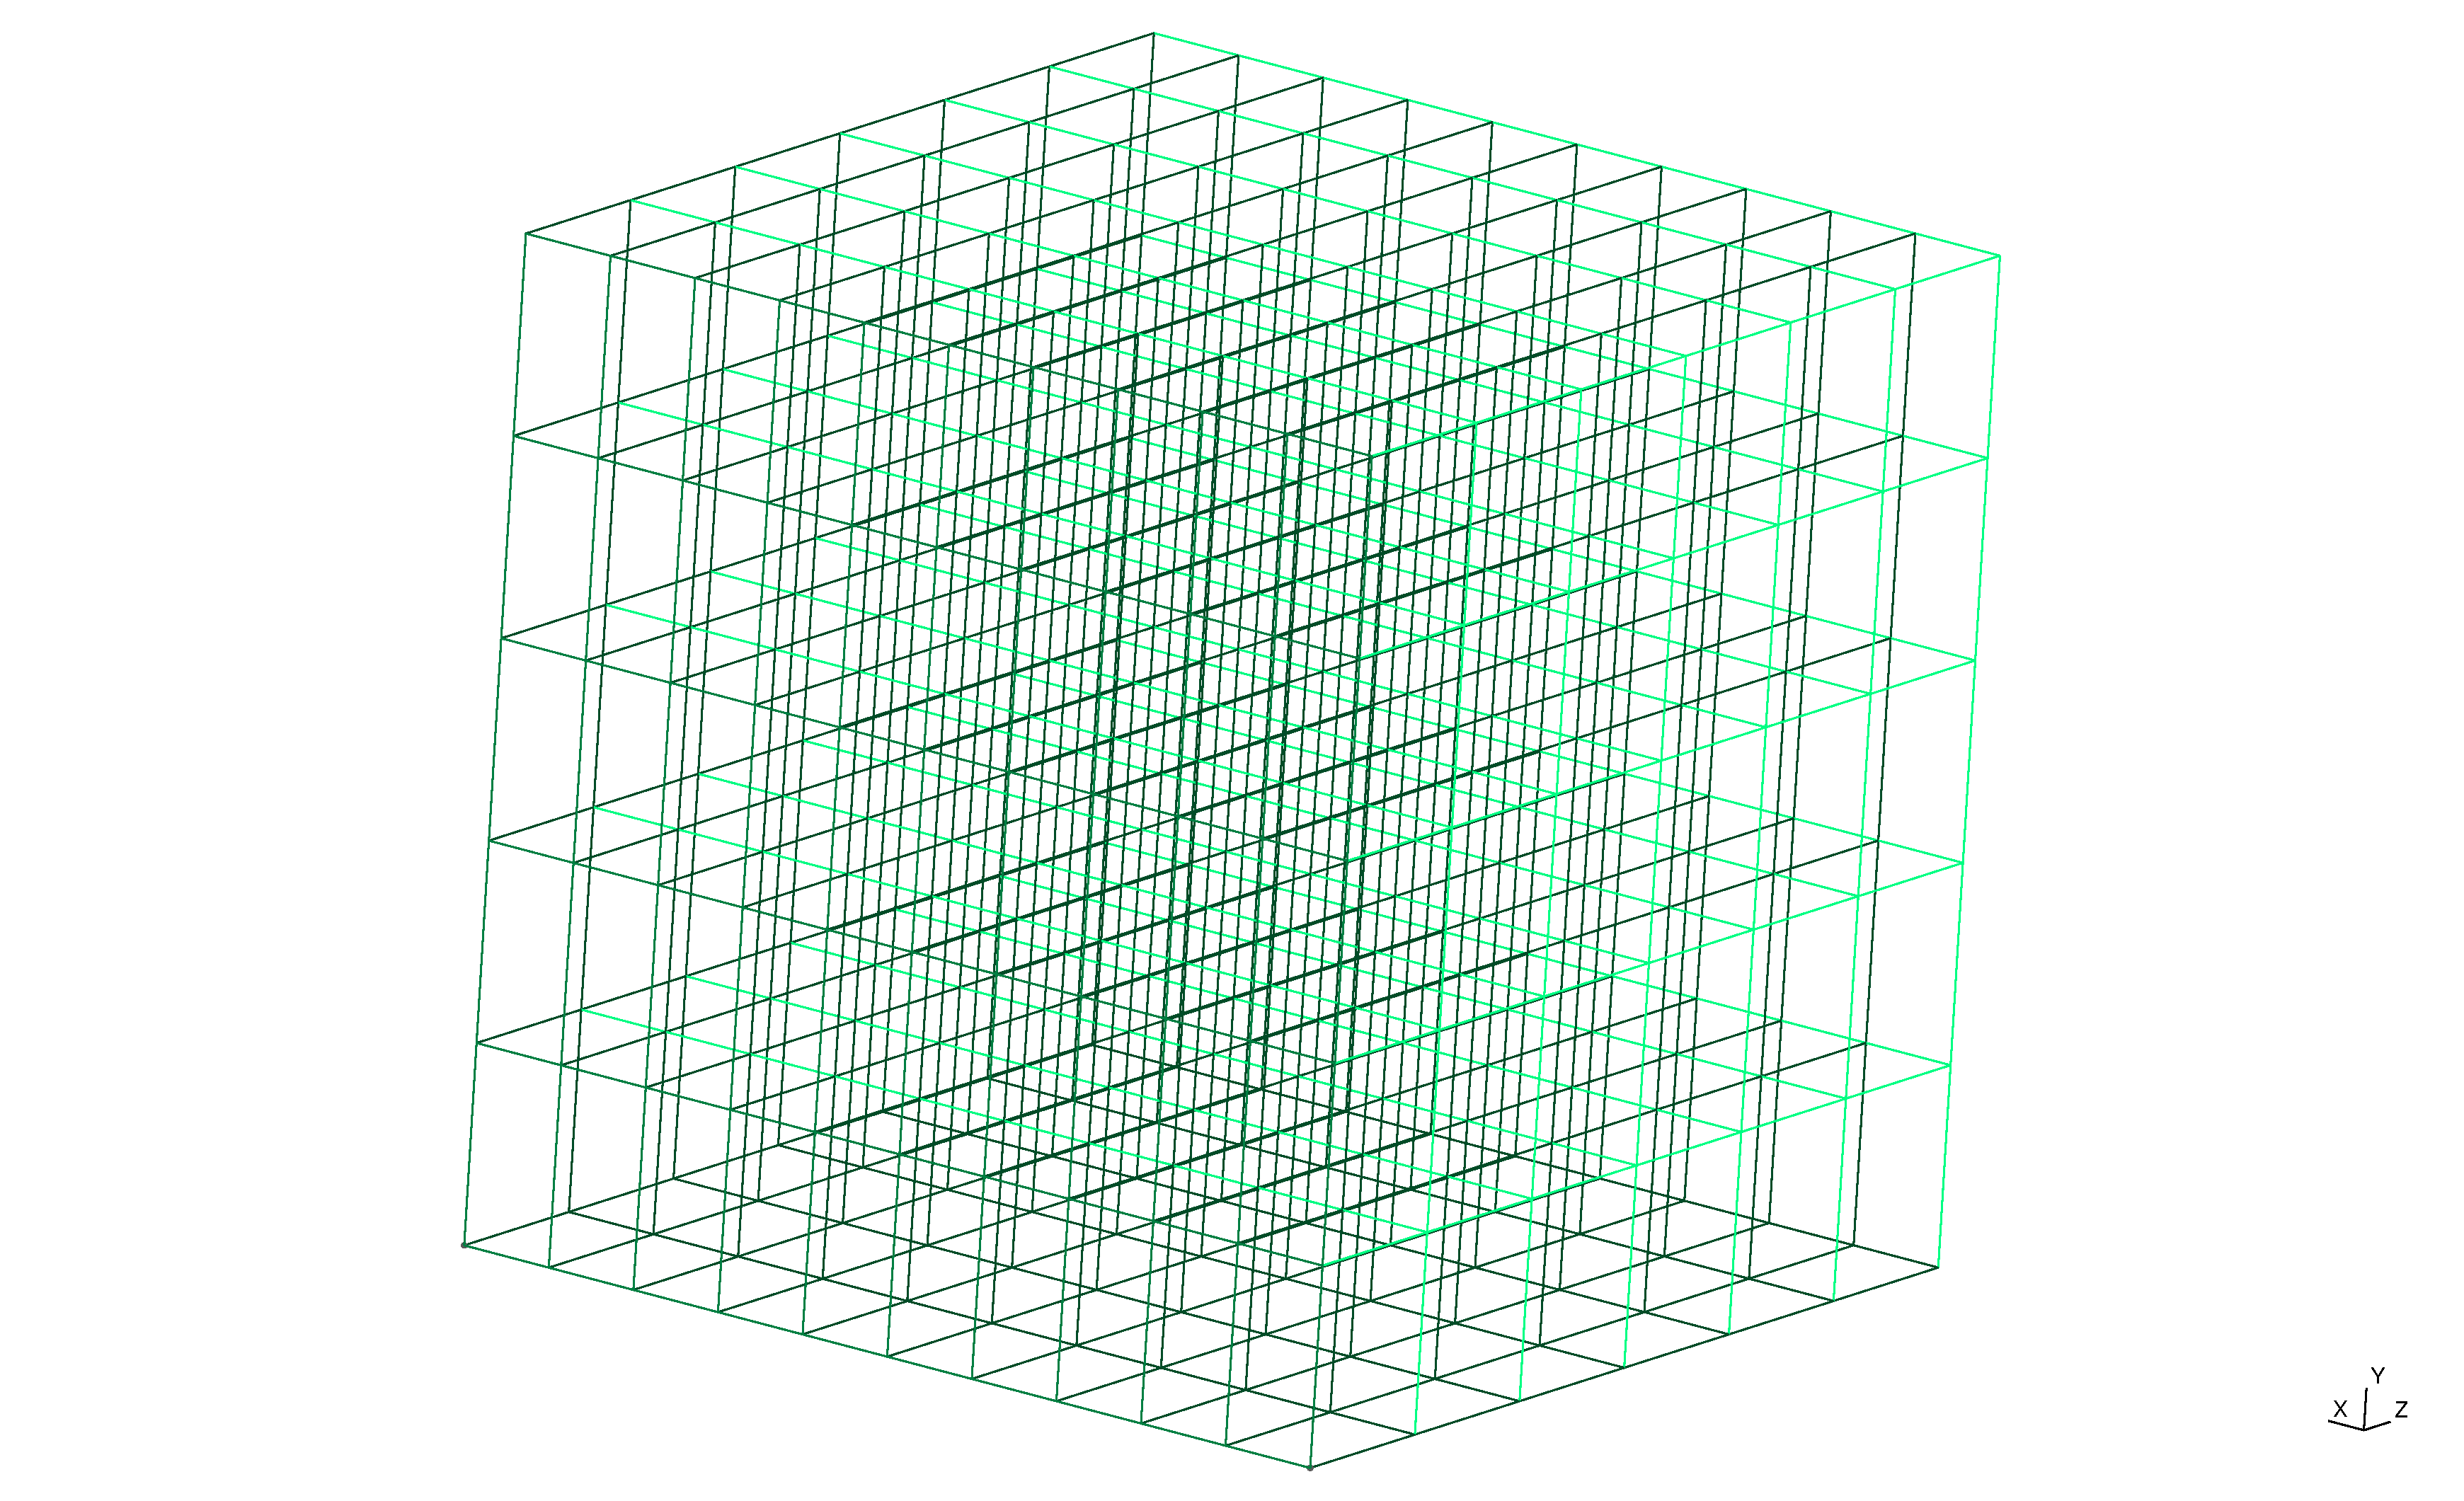
\includegraphics[width=0.45\textwidth]{cuboid.eps}
		}
\end{figure}
\subsection{与Easymesh的比较}
相比于AFEPack中使用的easymesh软件,Gmsh是一个成熟的网格剖分系统,
在网格剖分部分,二者
有以下一些差异之处:
\begin{itemize}
	\item Gmsh生成几何体的方式较为简便,可以通过一些基本元素的Extrude
		来生成。而Easymesh只能通过逐点描述线段来生成。
	\item Easymesh只能处理多边形边界的区域,
		Gmsh可以处理维带圆弧或者其余
		二次曲线的区域。例如在之前给出的有“ZLC”字样的区域,、
		就无法通过Easymesh进行剖分,只能先人为地用多边形去逼近这块区域
		,再交给easymesh剖分。
	\item Gmsh可以比较容易地设置网格在某个特定区域内稠密。
	\item 对于二维问题,Easymesh只能生成无结构三角形网格,Gmsh可以生成
		无结构的三角形、四边形以及结构三角形、四边形网格。
	\item Gmsh能够处理三维问题。
\end{itemize}
\newpage
\section{网格输出文件的结构分析}
通过在图形界面下的Save mesh,或是直接在终端下~\verb|gmsh %.geo -D|~,
可以将网格进行剖分并存入文件\%.msh。以下我们分析msh文件的格式:
\inputccode{sample.msh}
需要注意的是这里的结构性质参数,它的意义如下:
\begin{table}[H]
	\centering
	\begin{tabular}{|c|c|}
		结构性质参数 & 结构类型 \\
		1 & 2个节点的线段 \\
		2 & 3个节点的三角形  \\
		3 & 4个节点的四边形 \\
		4 & 4个节点的四面体 \\
		5 & 8个节点的六面体 \\
		6 & 6个节点的三棱柱 \\
		7 & 5个节点的四棱锥 \\
		15 &  1个节点的点 
	\end{tabular}
	\caption{结构类型}
\end{table}
我们这里不关心tag的意义。

以这份省略版的sample.msh为例,它描述了一个一共只有13个节点的网格。
这个结构体一共有28个结构,其中1-4号为点(结构性质参数
为15),
之后为边(结构性质参数为1),再之后为三角形(结构性质参数为2)。
因此这是一个三角形网格,且每个三角形网格的顶点都在
对应行的末尾给出(位于tag之后)。
\newpage
\section{有限元问题的求解}
\subsection{AFEPack对Gmsh的接口}
在AFEPack头文件中,有一个Mesh类,是AFEPack可以直接处理的网格形式,
这种形式的数据无法由gmsh的网格文件.msh文件直接得到。从而AFEPack为Gmsh
写了一个接口类GmshMesh
\footnote{AFEPack源代码这部分有一些小问题
,经过唐凤阳师兄修复之后可以使用},用于读入.msh文件并转化为Mesh类的形
式。

AFEPack中给出了六面体、三棱柱等几何体的模板单元,
但目前尚未给出能够正确处理Gmsh中对应形状网格的函数。
目前能够在AFEPack中使用的网格形式只有二维的三角形、四边形网格和三维
的四面体网格。

\subsection{一个简单的例子}
我们这里采用AFEPack来进行有限元问题的求解。事实上,AFEPack在读取网格时
已经为Gmsh写了接口,这里我们使用AFEPack读取一个简单的Gmsh网格,并求解
一个简单的泊松方程。\par
我们选取的区域是一个单位正方形减去中间的一个圆形区域,这是一个Easymesh
无法处理的区域形状。
具体方程和真实解为:
\[
-\Delta u = 5\pi^2\sin(\pi x)\sin(2\pi y)
\]
\[
 u = \sin(\pi x)\sin(2\pi y)
\]
边界条件采用狄利克雷边界条件。

利用AFEPack计算的结果显示如下:
\begin{figure}[H]
	\begin{center}
		\includegraphics[width=0.9\textwidth]{result.png}
	\end{center}
	\caption{AFEPack解泊松方程}
\end{figure}
其中与真解比较,L2误差为0.00013,可以认为AFEPack正确解决了这个问题。

通过这个简单的例子,我们搭建了从Gmsh剖分网格,到AFEPack
解决有限元问题的桥梁,使AFEPack摆脱了对Easymesh的依赖,
从而可以处理一些更复杂的区域问题和构建更适用的网格。
\newpage
\section{总结}
本次上次作业,我们学习了网格剖分软件Gmsh,这是一款网格剖分的专业软件。
相比Easymesh,Gmsh的适用范围更大,生成几何体
的方式更简单,而且能够处理三维的几何结构以及曲线形状的
几何体,还能剖分出三角形,四边形,四面体网格和各种结构网格。

此外,我们还利用了AFEPack软件包以及它对Gmsh的接口,求解了一个简单的二
维区域的泊松方程,取得了不错的结果。目前AFEPack可以用于求解二维的Gmsh网
格,以及三维的Gmsh生成的四面体网格。其他形状的网格暂时还没有支持的接口
。

此次上机作业只记录了一些Gmsh的基本用法,还有待更进一步的学习。
Gmsh官方提供的帮助文档十分详细,下载地址为
http://gmsh.info/doc/texinfo/gmsh.pdf. 


\end{document}


